\documentclass[english,11pt]{beamer}
%%%%%%%%%%%%%%%%%%%%%%%%%%%%%
% Standard header for working papers
%
% WPHeader.tex
%
%%%%%%%%%%%%%%%%%%%%%%%%%%%%%

\documentclass[11pt]{article}



%%%%%%%%%%%%%%%%%%%%%%%%%%
%% TEMPLATES
%%%%%%%%%%%%%%%%%%%%%%%%%%


% Simple Tabular

%\begin{tabular}{ |c|c|c| } 
% \hline
% cell1 & cell2 & cell3 \\ 
% cell4 & cell5 & cell6 \\ 
% cell7 & cell8 & cell9 \\ 
% \hline
%\end{tabular}





%%%%%%%%%%%%%%%%%%%%%%%%%%
%% Packages
%%%%%%%%%%%%%%%%%%%%%%%%%%



% encoding 
\usepackage[utf8]{inputenc}
\usepackage[T1]{fontenc}


% general packages without options
\usepackage{amsmath,amssymb,amsthm,bbm}

% graphics
\usepackage{graphicx,transparent,eso-pic}

% text formatting
\usepackage[document]{ragged2e}
\usepackage{pagecolor,color}
%\usepackage{ulem}
\usepackage{soul}


% conditions
\usepackage{ifthen}


\usepackage{natbib}


%%%%%%%%%%%%%%%%%%%%%%%%%%
%% Maths environment
%%%%%%%%%%%%%%%%%%%%%%%%%%

%\newtheorem{theorem}{Theorem}[section]
%\newtheorem{lemma}[theorem]{Lemma}
%\newtheorem{proposition}[theorem]{Proposition}
%\newtheorem{corollary}[theorem]{Corollary}

%\newenvironment{proof}[1][Proof]{\begin{trivlist}
%\item[\hskip \labelsep {\bfseries #1}]}{\end{trivlist}}
%\newenvironment{definition}[1][Definition]{\begin{trivlist}
%\item[\hskip \labelsep {\bfseries #1}]}{\end{trivlist}}
%\newenvironment{example}[1][Example]{\begin{trivlist}
%\item[\hskip \labelsep {\bfseries #1}]}{\end{trivlist}}
%\newenvironment{remark}[1][Remark]{\begin{trivlist}
%\item[\hskip \labelsep {\bfseries #1}]}{\end{trivlist}}

%\newcommand{\qed}{\nobreak \ifvmode \relax \else
%      \ifdim\lastskip<1.5em \hskip-\lastskip
%      \hskip1.5em plus0em minus0.5em \fi \nobreak
%      \vrule height0.75em width0.5em depth0.25em\fi}



%% Commands

\newcommand{\noun}[1]{\textsc{#1}}


%% Math

% Operators
\DeclareMathOperator{\Cov}{Cov}
\DeclareMathOperator{\Var}{Var}
\DeclareMathOperator{\E}{\mathbb{E}}
\DeclareMathOperator{\Proba}{\mathbb{P}}

\newcommand{\Covb}[2]{\ensuremath{\Cov\!\left[#1,#2\right]}}
\newcommand{\Eb}[1]{\ensuremath{\E\!\left[#1\right]}}
\newcommand{\Pb}[1]{\ensuremath{\Proba\!\left[#1\right]}}
\newcommand{\Varb}[1]{\ensuremath{\Var\!\left[#1\right]}}

% norm
\newcommand{\norm}[1]{\left\lVert #1 \right\rVert}



% argmin
\DeclareMathOperator*{\argmin}{\arg\!\min}


% amsthm environments
\newtheorem{definition}{Definition}
\newtheorem{proposition}{Proposition}
\newtheorem{assumption}{Assumption}

%% graphics

% renew graphics command for relative path providment only ?
%\renewcommand{\includegraphics[]{}}


\usepackage{url}





% geometry
\usepackage[margin=2cm]{geometry}



% changes

\usepackage{soul}
\soulregister\cite7
\soulregister\citep7
\soulregister\ref7

\usepackage[final]{changes}
%\usepackage{changes}


\setaddedmarkup{\textcolor{black}{\hl{#1}}}
\setdeletedmarkup{\textcolor{red}{\sout{#1}}}



\usepackage{CJKutf8}
%\begin{CJK*}{UTF8}{zhsong}
%文章内容。
%\clearpage\end{CJK*}
\newcommand{\cn}[1]{
  \begin{CJK*}{UTF8}{gbsn}
  #1
  \end{CJK*}
}



% layout : use fancyhdr package
%\usepackage{fancyhdr}
%\pagestyle{fancy}
%
%\makeatletter
%
%\renewcommand{\headrulewidth}{0.4pt}
%\renewcommand{\footrulewidth}{0.4pt}
%\fancyhead[RO,RE]{}
%\fancyhead[LO,LE]{Models for the co-evolution of cities and networks}
%\fancyfoot[RO,RE] {\thepage}
%\fancyfoot[LO,LE] {}
%\fancyfoot[CO,CE] {}
%
%\makeatother
%

%%%%%%%%%%%%%%%%%%%%%
%% Begin doc
%%%%%%%%%%%%%%%%%%%%%

\begin{document}









\title{Caractérisation et modélisation de la co-évolution\\
des réseaux de transport et des territoires}

\author{J.~Raimbault$^{1,2,3,\ast}$\\
\texttt{juste.raimbault@iscpif.fr}
}


\institute{$^{1}$UPS CNRS 3611 ISC-PIF\\
$^{3}$CASA,UCL\\
$^{2}$UMR CNRS 8504 G{\'e}ographie-cit{\'e}s
}


\date{Prix de Thèse Systèmes Complexes\\\smallskip
Lundi 17 juin 2019\\\smallskip
Institut des Systèmes Complexes
}

\frame{\maketitle}


\sframe{Contexte scientifique}{


\begin{columns}


	\begin{column}{0.5\textwidth}

	\begin{center}
	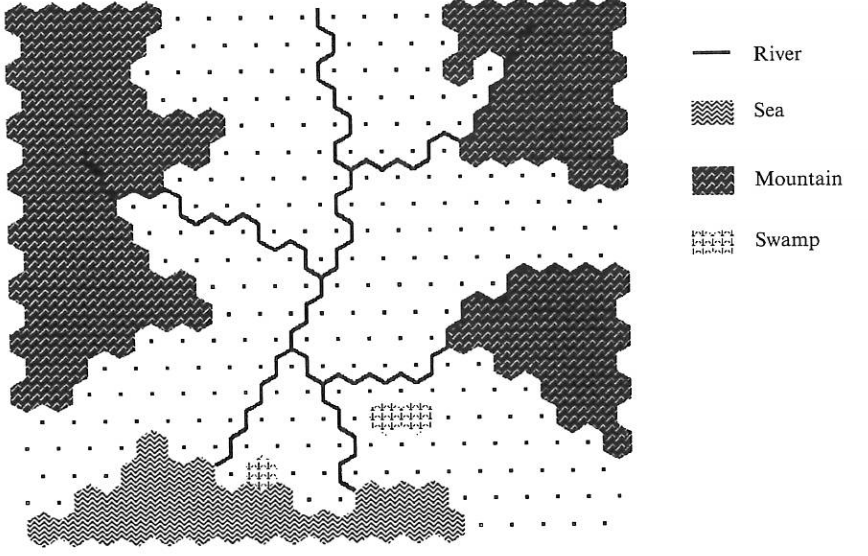
\includegraphics[width=0.7\textwidth]{figures/simpop1.png}
	\end{center}
	
	
	\footnotesize
\textit{Simpop 1 model \cite{sanders1997simpop}}

	\medskip

	\hrule
	
	

\begin{center}
	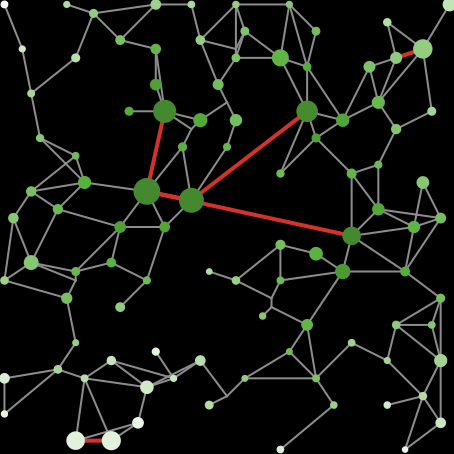
\includegraphics[width=0.5\textwidth]{figures/setup_synth_1_tick100.png}
	\end{center}
	
	\footnotesize
	\textit{SimpopNet model \cite{schmitt2014modelisation}}
	
	\end{column}

 \vrule{}

\begin{column}{0.5\textwidth}
	
	\vspace{-1cm}
	\begin{center}
	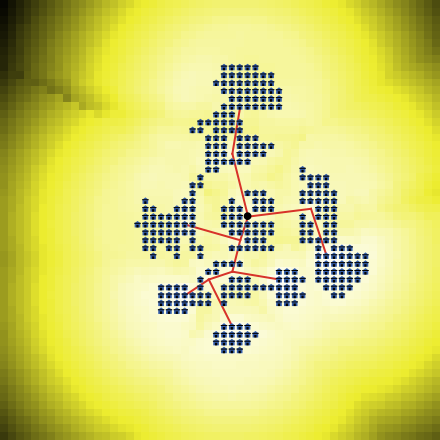
\includegraphics[width=0.55\textwidth,height=0.3\textheight]{figures/intro_RBD_lattice.png}
	\end{center}
	
	
	\footnotesize
\textit{Hybrid urban morphogenesis \cite{raimbault2014hybrid}}
	
	
	\medskip
	\hrule
	\medskip

	
	\begin{center}
	
\includegraphics[width=0.55\textwidth]{figures/openmole.png}
	\end{center}
	
	\footnotesize
\textit{Nouvelles méthodes d'exploration des modèles de simulation \cite{reuillon2013openmole}}
	

	\end{column}

\end{columns}

}





\sframe{Interactions entre réseaux et territoires}{

\justify

\begin{center}

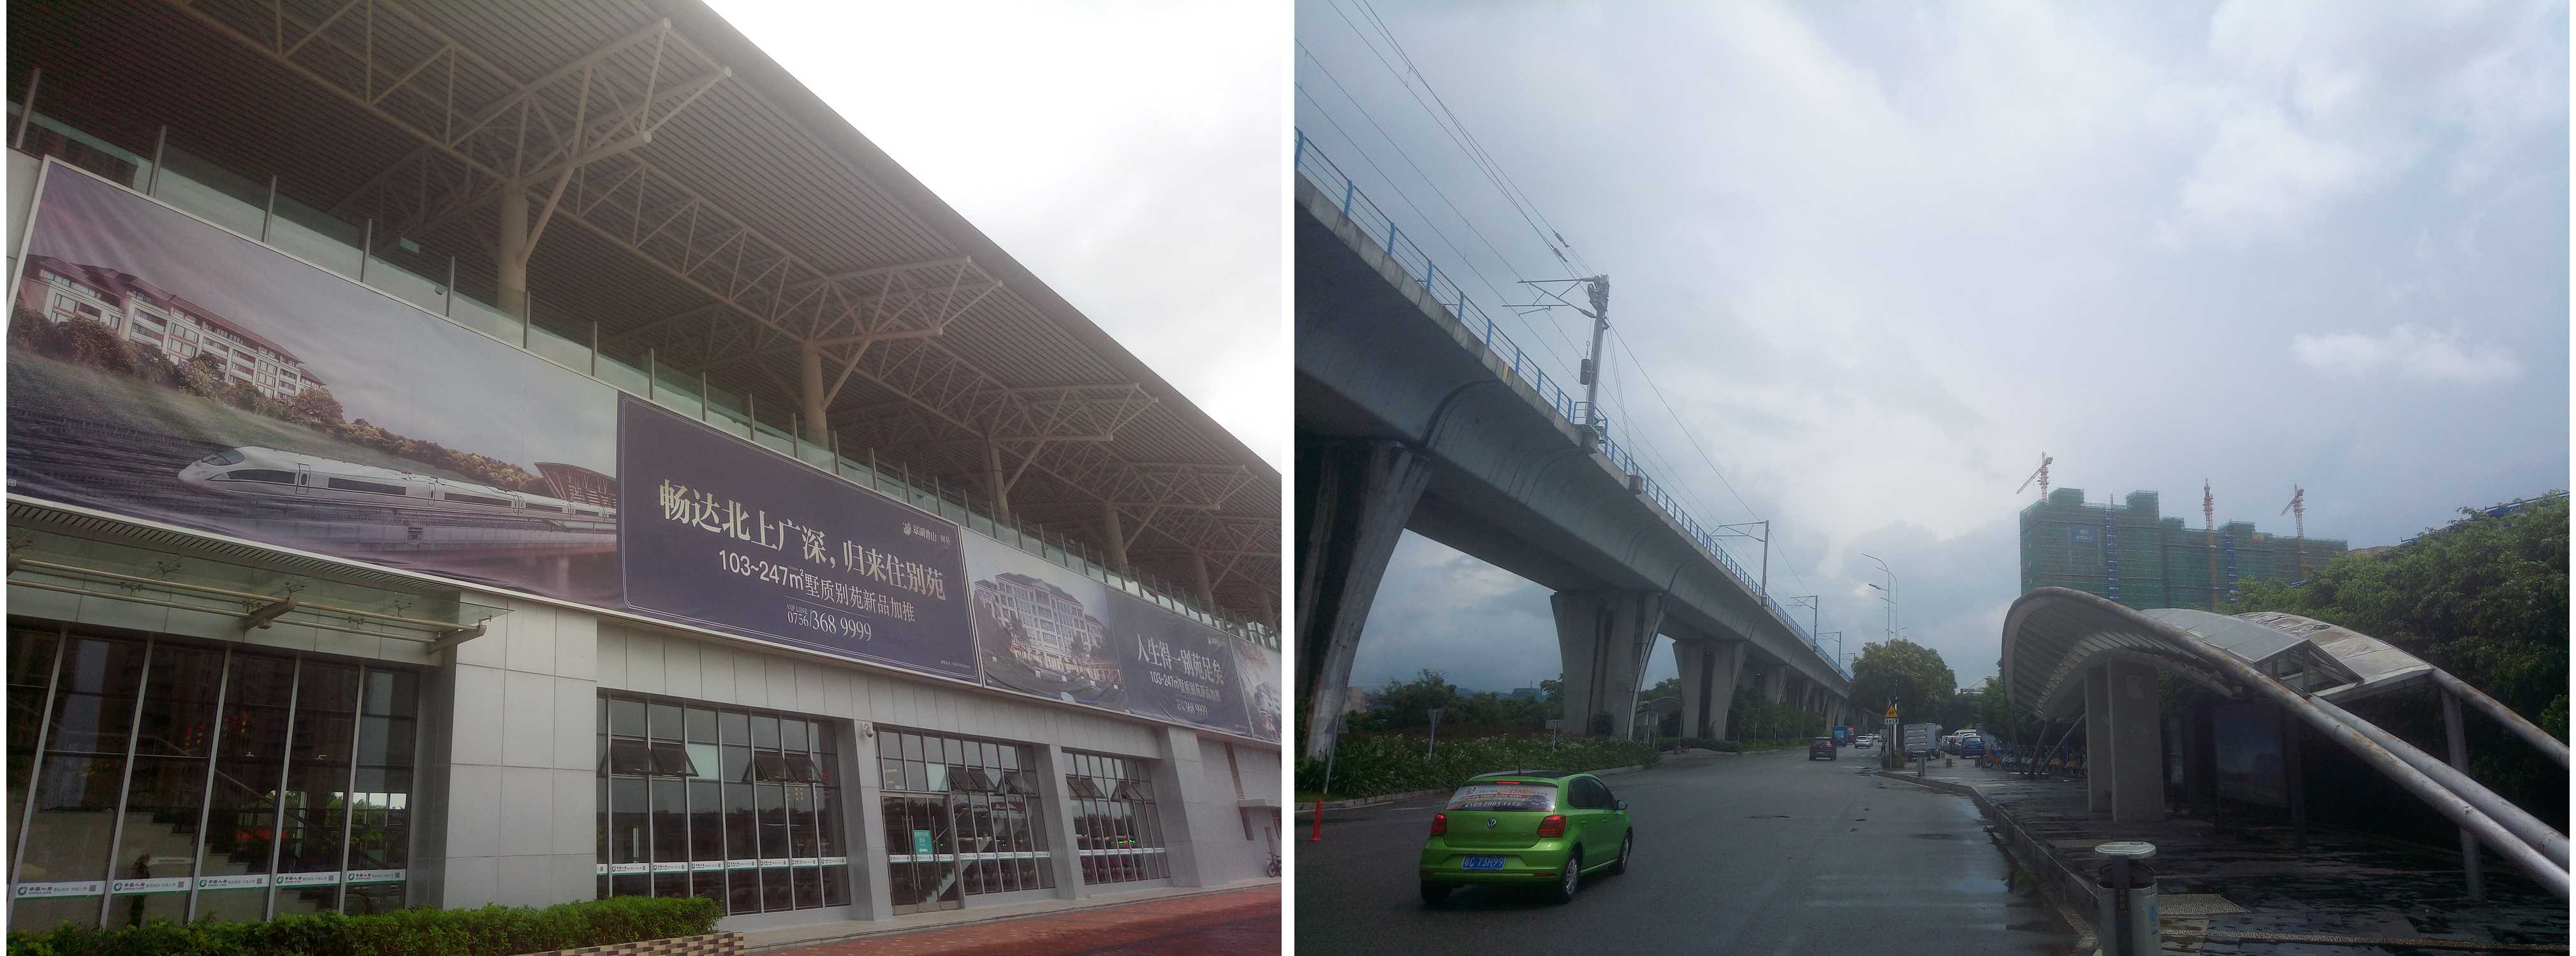
\includegraphics[width=\linewidth]{figures/example-tangjia.jpg}

\end{center}

\medskip

%\vspace{-0.5cm}

%\begin{justify}
\textit{Observation d'interactions entre transport et ville dans le Delta de la Rivière des Perles : promotion de la grande vitesse, développement urbain ciblé autour des gares.}
%\end{justify}

\nocite{raimbault2018evolving}

\medskip

\tiny

Raimbault, J. (2019). Evolving accessibility landscapes: mutations of transportation networks in China. In Aveline-Dubach, N., ed. \textit{Pathways of sustainable urban development across China - the cases of Hangzhou, Datong and Zhuhai}, pp 89-108. Imago. ISBN:978-88-94384-71-0

}



\sframe{Problématique de la thèse}{


Des dynamiques \textit{co-évolutives} entre réseaux de transport et territoires suggérées par de nombreux travaux (Théorie Evolutive des Villes).

\bigskip

\textbf{Axe 1 : } \textit{Comment définir et caractériser empiriquement ces dynamiques co-évolutives ?}

\bigskip

$\rightarrow$ Connaissance par les seules études empiriques qui reste limitée.
%(données pauvres, cas d'étude, temps long, couplage fort).

\bigskip

\textbf{Axe 2 : } \textit{Comment modéliser la co-évolution des réseaux de transport et des territoires ?}

\bigskip

$\rightarrow$ Utilisation de la modélisation comme outil de connaissance.


}


\sframe{Vers une modélisation ? Cartographie des disciplines}{
	
	\footnotesize
	
	\textit{Multiples points de vue sur les mêmes objets,
	 modélisations complémentaires.}
	
%	\vspace{-0.5cm}
	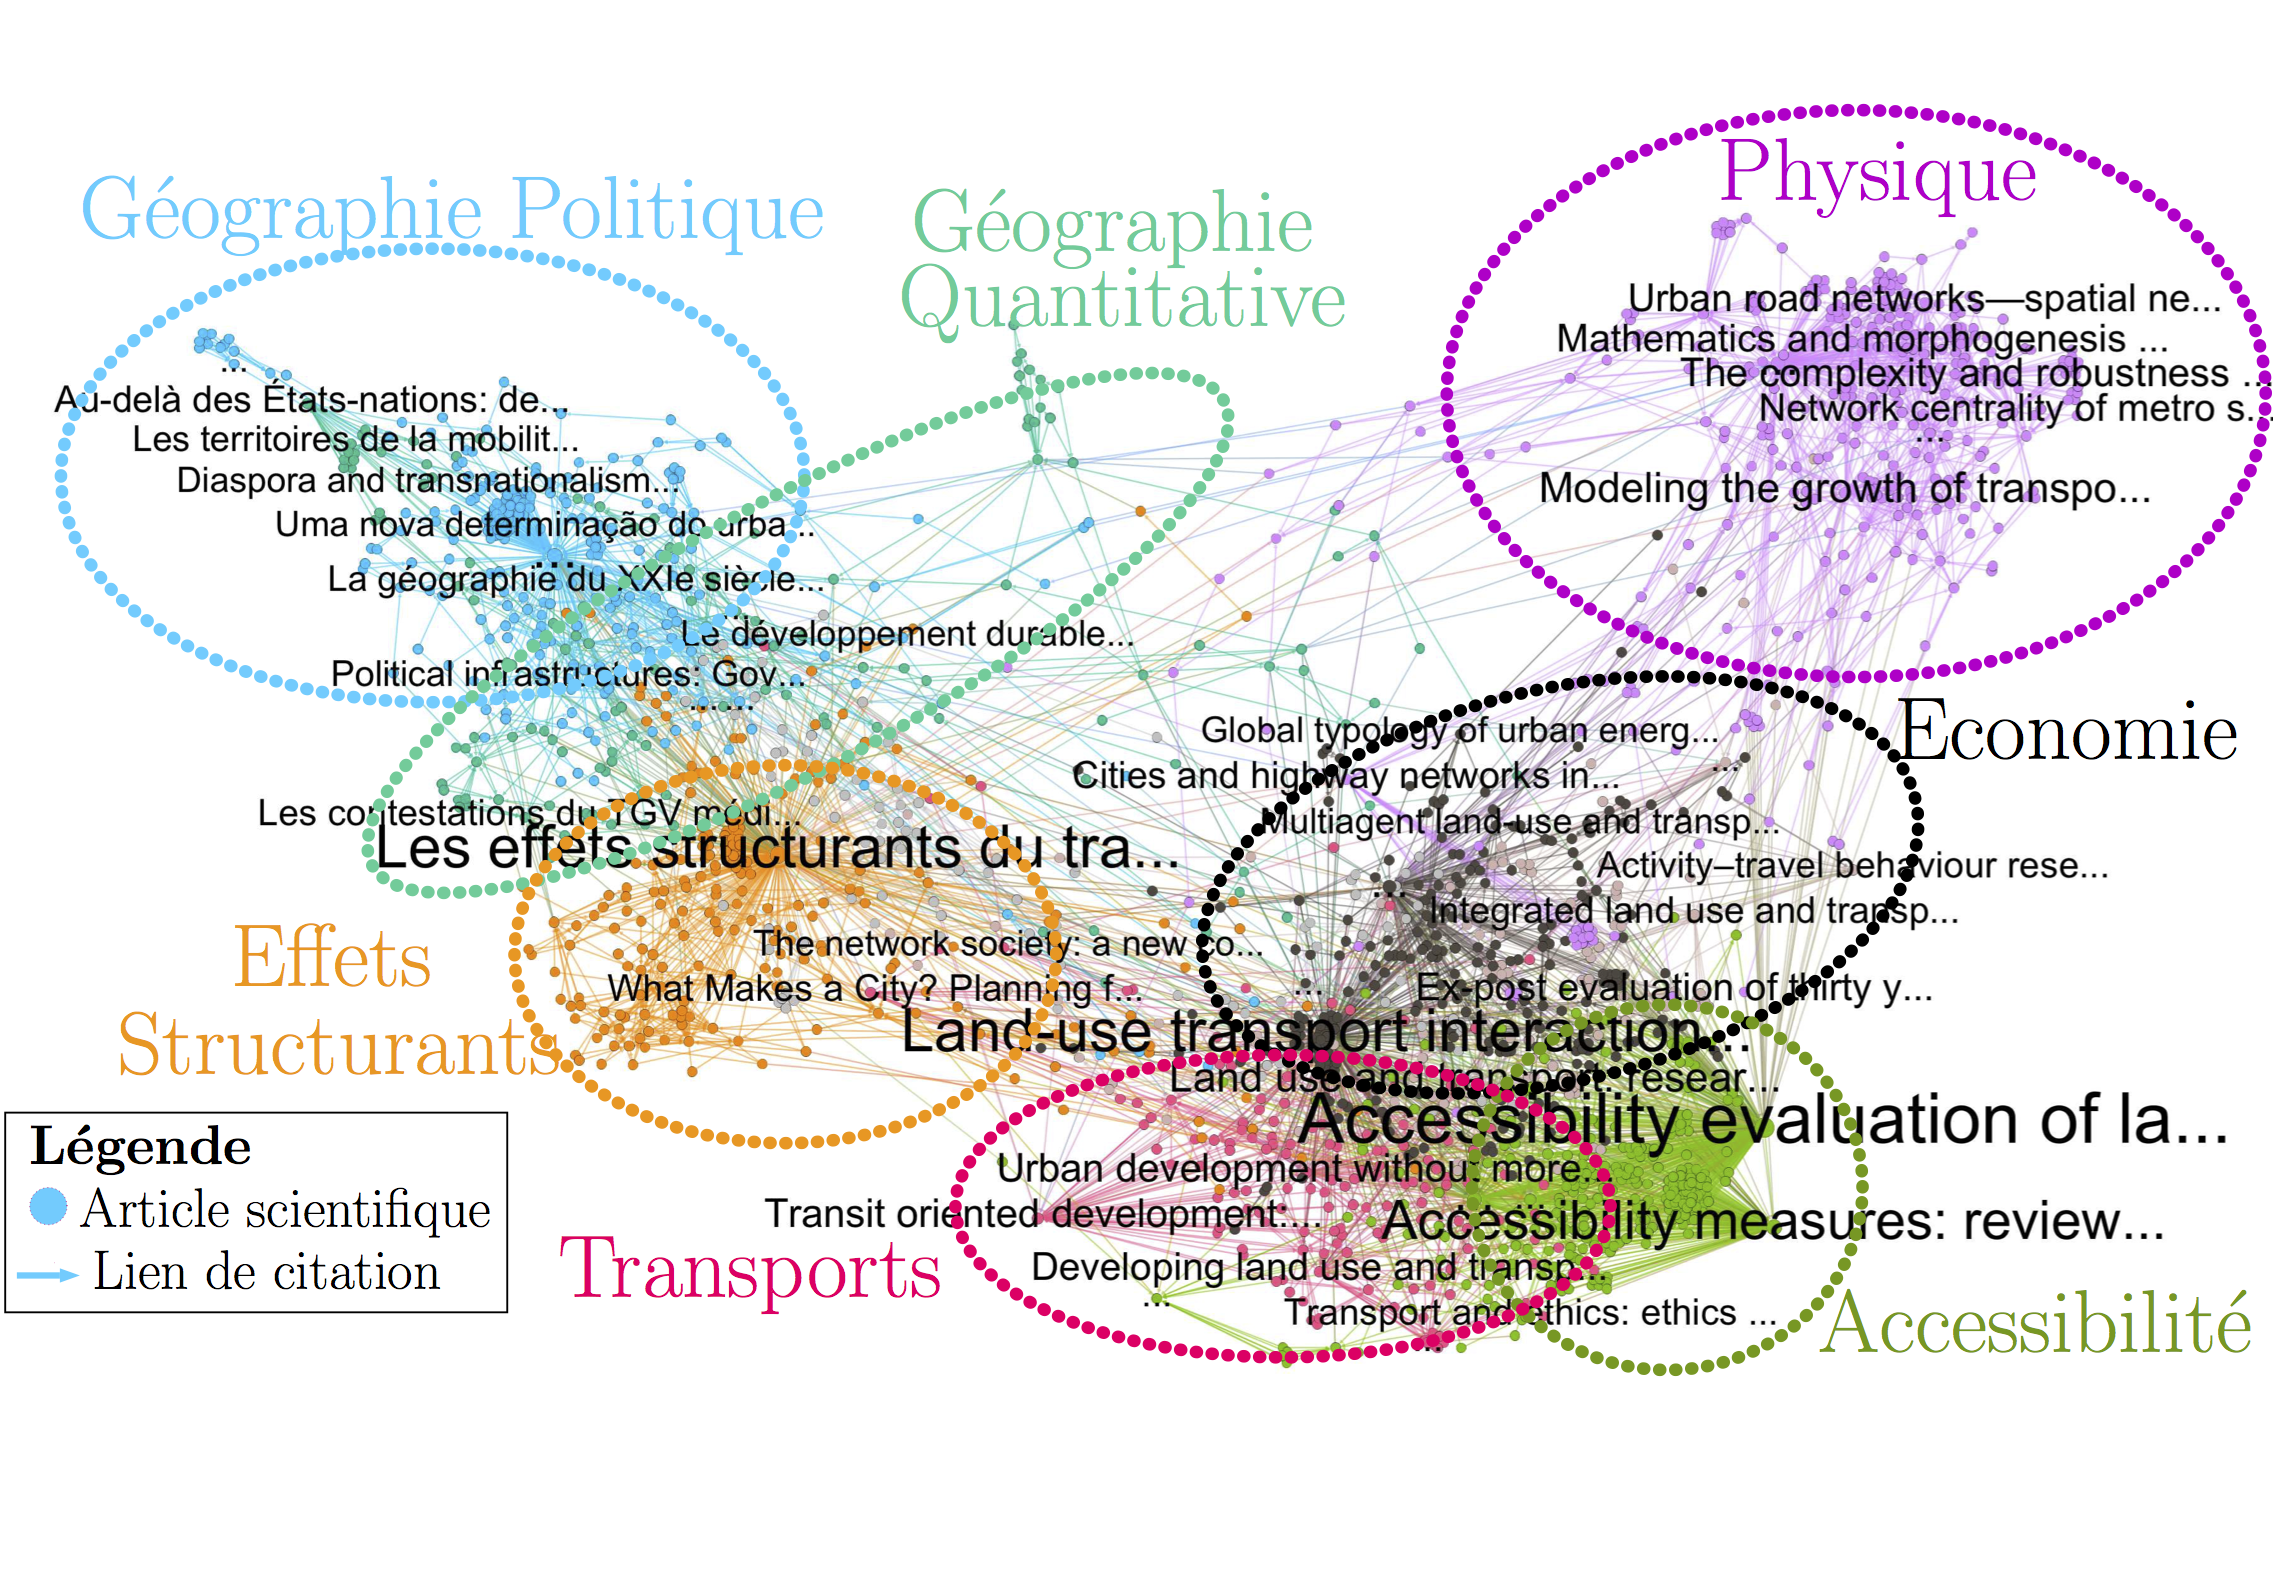
\includegraphics[width=0.9\linewidth,trim={0 2cm 0 2cm},clip]{figures/quantep-graph.png}

	 
	 \footnotesize
	 
	 %\vspace{-0.5cm}
	 
	 \nocite{raimbault2019exploration}
	 
	 Raimbault, J. (2019). Exploration of an interdisciplinary scientific landscape. Scientometrics, 1-25.
	 
	 
}



\begin{frame}
	\frametitle{Lecture par les domaines de connaissance}
	\begin{center}
	\vspace{-0.8cm}
	\begin{tikzpicture}
		\node (a) at (-1,1.5) {Empirique};
		\node (b) at (-1,0) {\includegraphics[width=2.5cm]{figures/domconn-empirical.png}};
			\node (c) at (3,5) {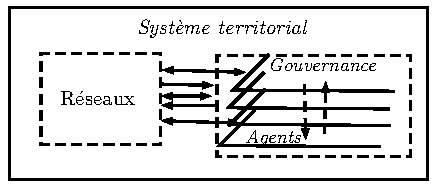
\includegraphics[width=4.5cm]{figures/domconn-schema.pdf}};
			\node (d) at (3,3.5) {Théorique};
			\node (e) at (7,1.5) {Modélisation};
			\node (f) at (7,0) {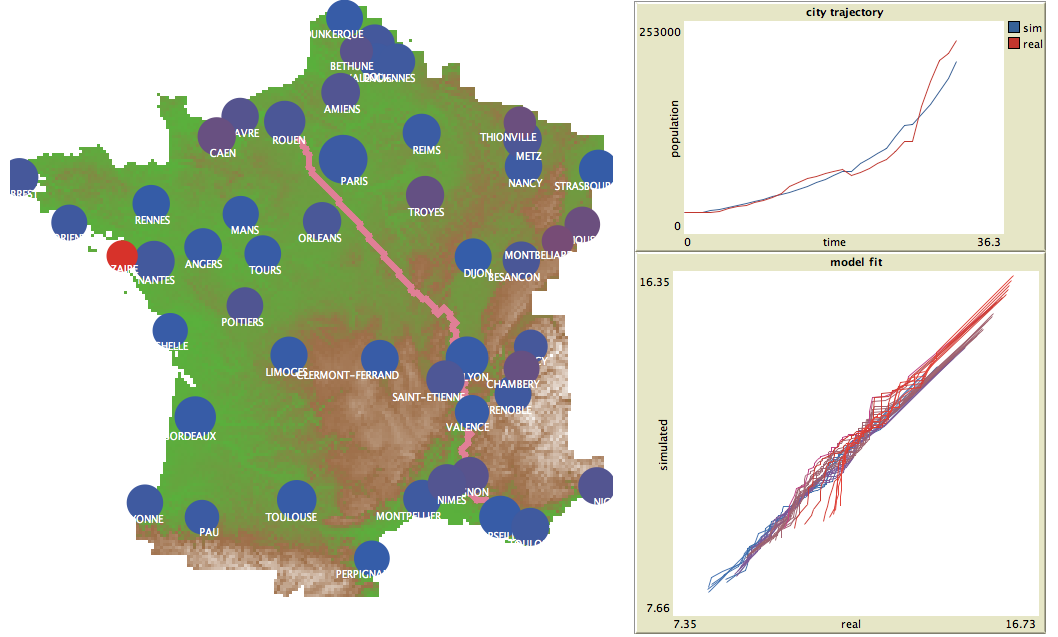
\includegraphics[width=3.5cm]{figures/domconn-modeling.png}};
			\draw[<->] (a) -- (d);
			\draw[<->] (d) -- (e);
			\draw[<->] (a) -- (e);
		\only<2->{
		\hspace{-0.5cm}
			\node (g) at (-1.5,5) {\textit{Méthodes}};
			\node (h) at (-1.5,4) {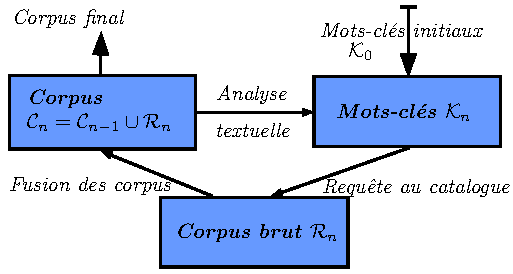
\includegraphics[width=3.5cm]{figures/domconn-methods.pdf}};
			\node (i) at (7.5,5) {\textit{Outils}};
			\node (j) at (7.2,3.8) {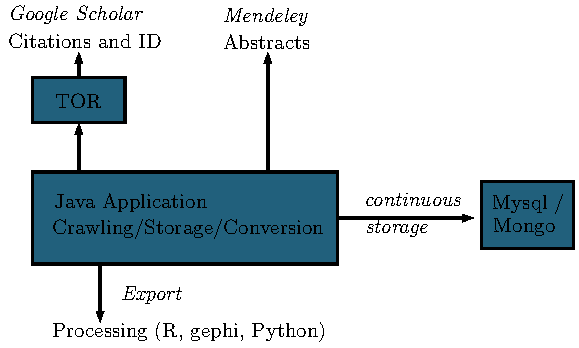
\includegraphics[width=3.2cm]{figures/domconn-tools.pdf}};
			\node (k) at (3,1) {\textit{Données}};
			\node (l) at (3,-0.5) {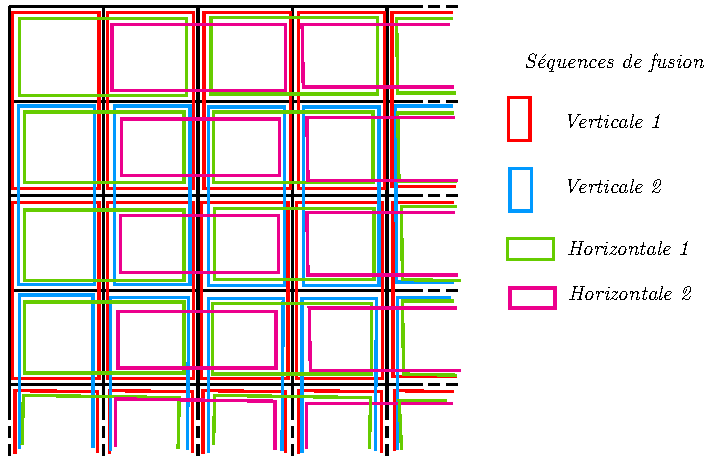
\includegraphics[width=3.5cm]{figures/domconn-data.pdf}};
		}
	\end{tikzpicture}
	
	\end{center}
	
	\vspace{-0.5cm}
	
	\footnotesize
	
	\nocite{raimbault2017applied}
	
	Raimbault, J. (2017). An Applied Knowledge Framework to Study Complex Systems. In Complex Systems Design \& Management (pp. 31-45).
	
	
	
\end{frame}


\sframe{Entrée théorique : définitions}{
 
  \textbf{Objets : } 
  
  \begin{itemize}
  	\item Villes et territoires lus au prisme de la \textit{Théorie Evolutive des Villes}
  	\item Réseaux de transport comme matérialisation de ``projets transactionnels'', suivant la \textit{Théorie Territoriale des Réseaux}
  \end{itemize}
 
 \bigskip

\uncover<2->{

\textbf{Processus : }

\textit{Une définition de la co-évolution à trois niveaux : } 
\begin{enumerate}
	\item \textcolor{blue}{niveau des agents}
	\item \textcolor{green}{niveau des populations d'agents (niches)}
	\item \textcolor{red}{niveau global du système}
\end{enumerate}  

}

\bigskip

\uncover<3->{

\textbf{Entrées : }

\begin{enumerate}
	\item \textcolor{blue}{Entrée empirique (niveau microscopique)}
	\item \textcolor{green}{Entrée par la morphogenèse (niveau de la niche)}
	\item \textcolor{red}{Entrée par la théorie évolutive (niveau global)}
\end{enumerate}

}
 
 
}


\sframe{Elaboration d'une méthode de caractérisation}{

\begin{center}
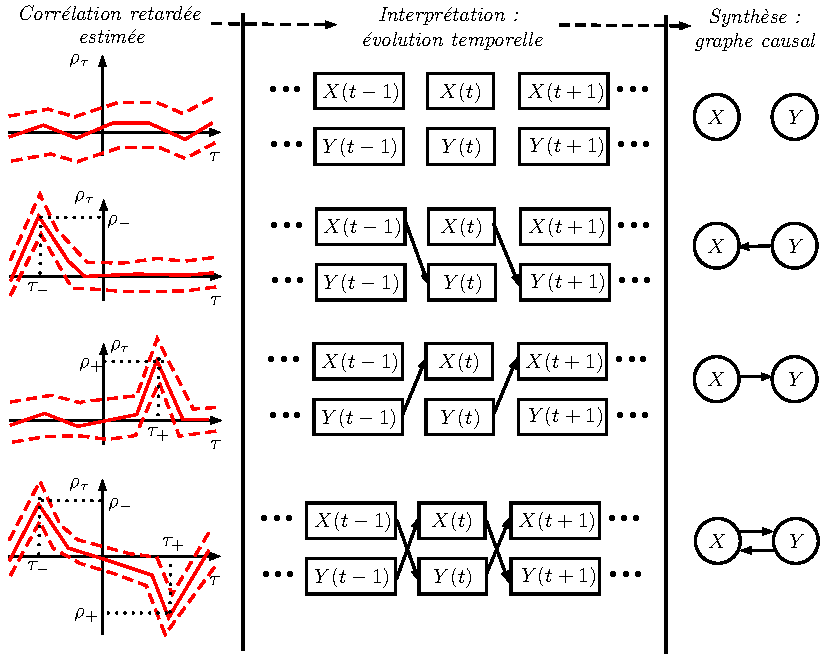
\includegraphics[width=0.8\linewidth]{figures/causality-method.pdf}
\end{center}


\tiny

\nocite{raimbault2017identification}

Raimbault, J. (2017). Identification de causalit{\'e}s dans des donn{\'e}es spatio-temporelles. In Spatial Analysis and GEOmatics 2017.

}



\sframe{Des observations empiriques contrastées}{

%Application de la méthode de caractérisation à des cas d'études à différentes échelles
%\bigskip

%\begin{columns}
%\begin{column}{0.5\textwidth}


	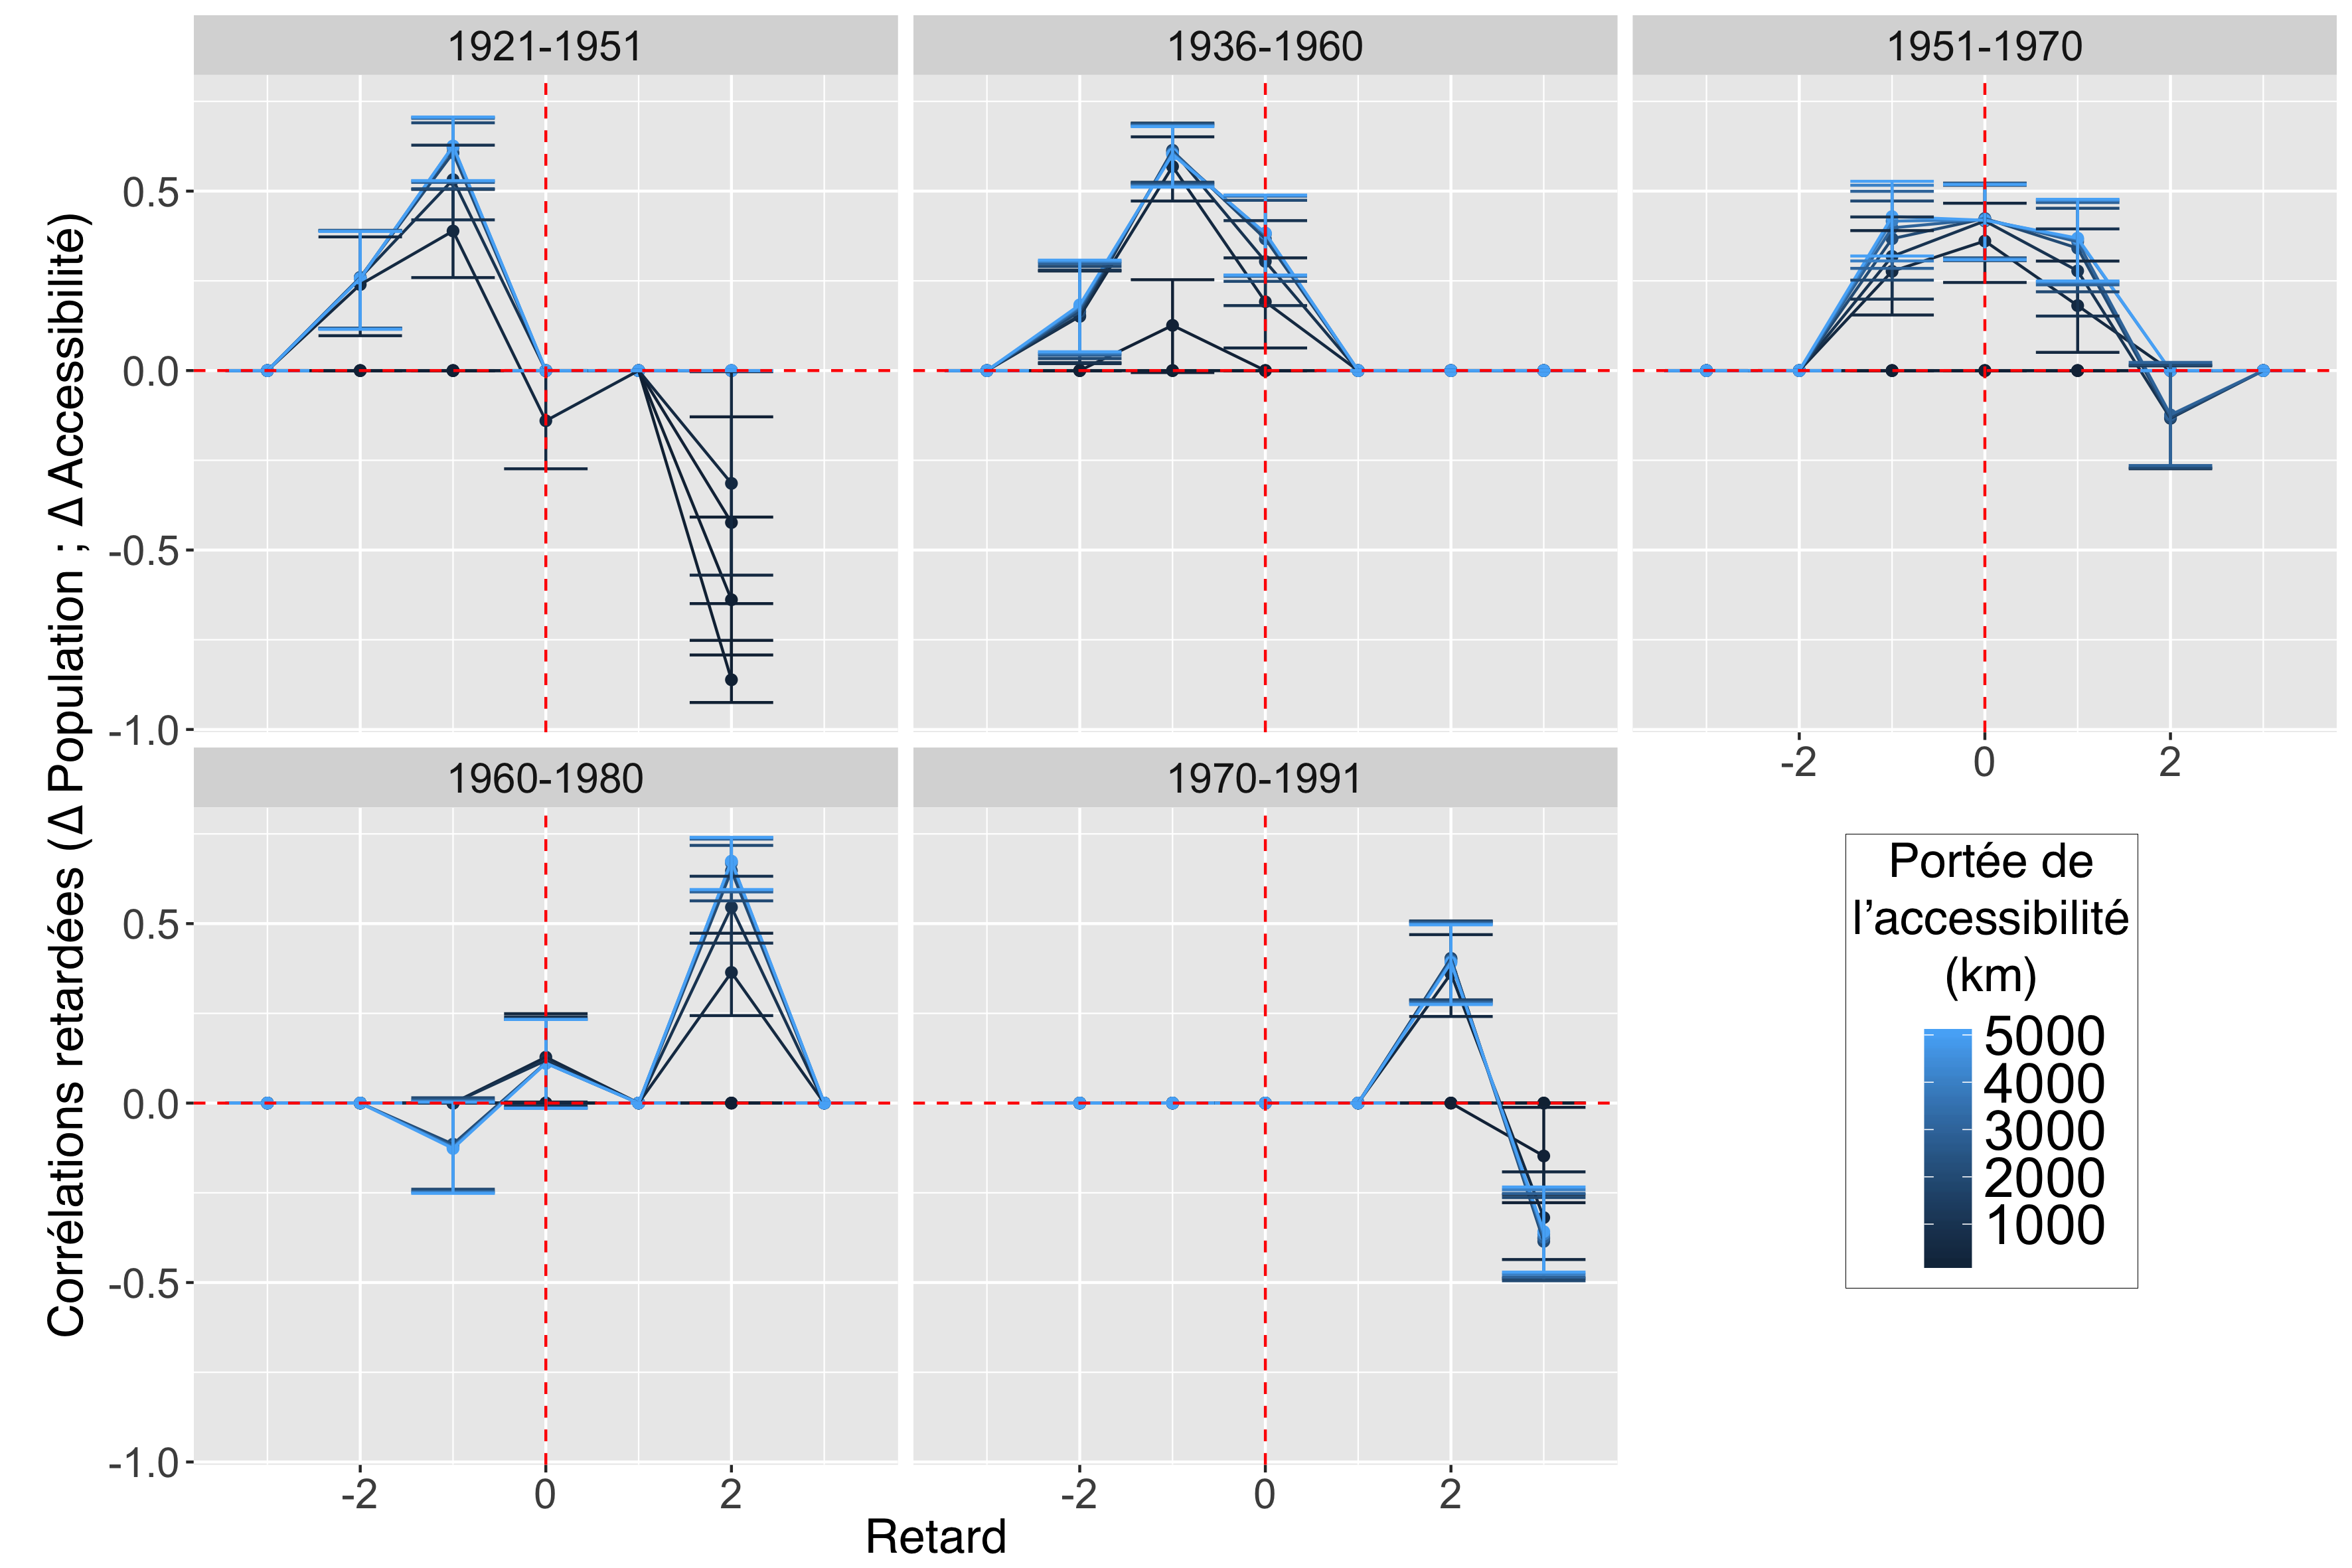
\includegraphics[width=\textwidth,height=0.8\textheight]{figures/empirical-southafrica.png}
	
	\smallskip
	
	
	\footnotesize
	
	%\vspace{-0.5cm}
	
	
	\begin{justify}
	\textit{Inversion du sens de la causalité entre croissance des populations et de l'accessibilité ferroviaire en Afrique du Sud au cours du 20ème siècle}
	\end{justify}


%\end{column}
%\vrule\hspace{0.2cm}
%	\begin{column}{0.45\textwidth}

}



\sframe{Des observations empiriques contrastées}{


\begin{center}
	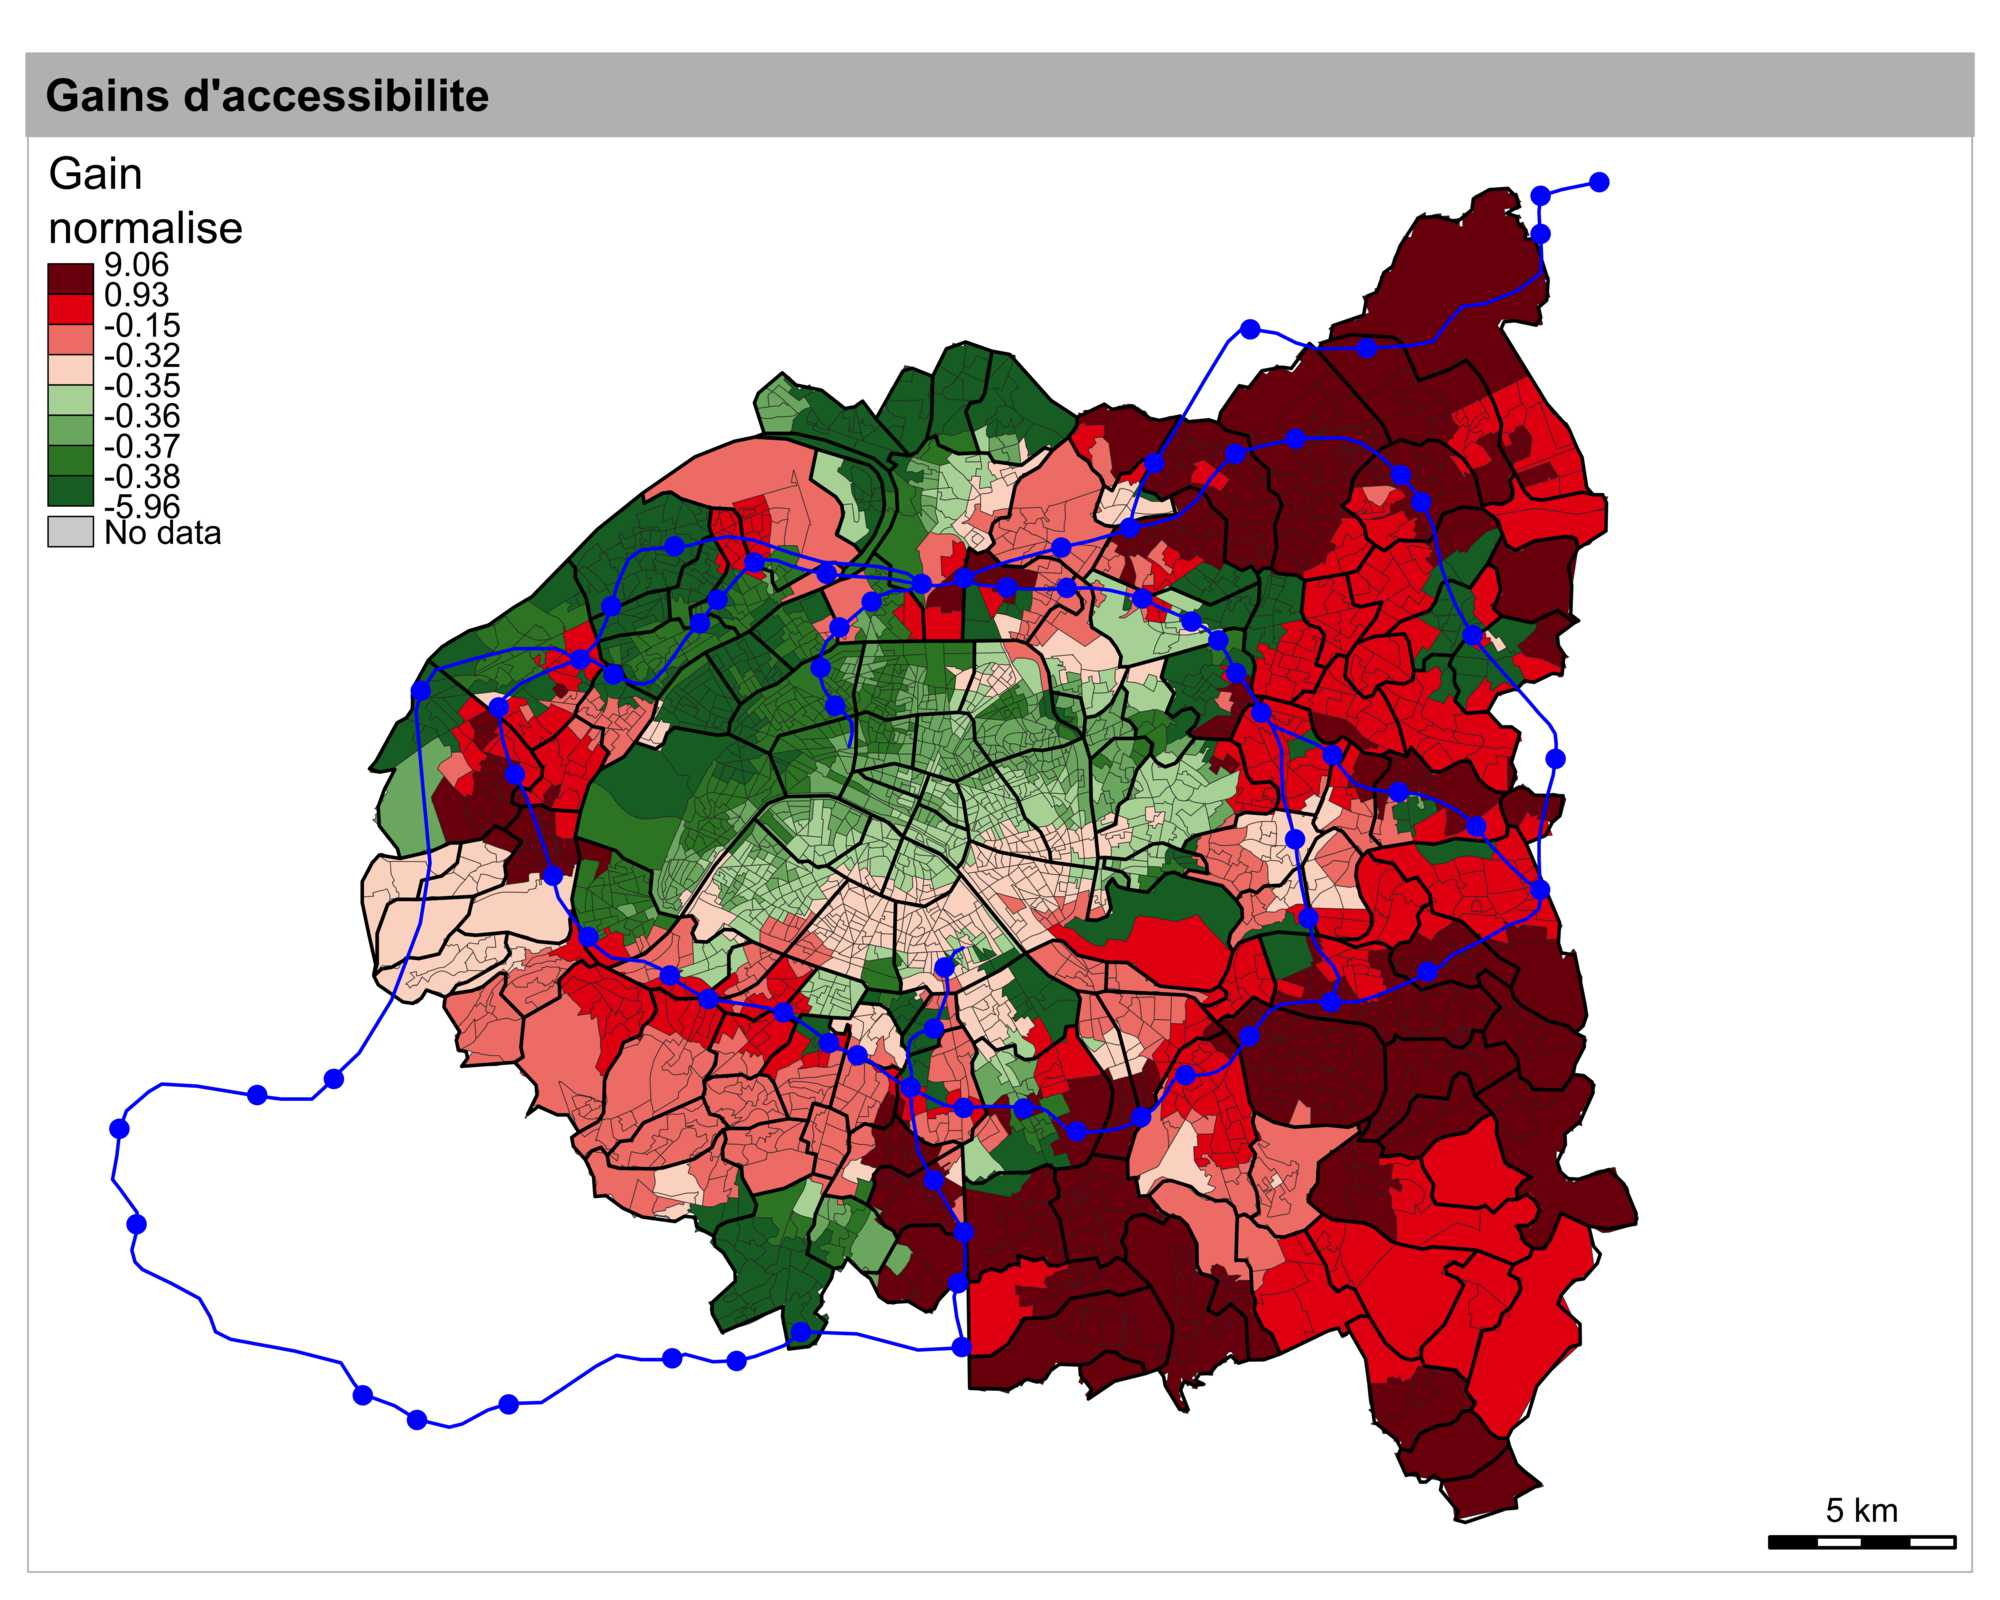
\includegraphics[width=0.8\textwidth]{figures/empirical-grdparis.jpg}
\end{center}	

	
	%\smallskip
	
	\footnotesize
	
	\vspace{-0.5cm}
	\begin{justify}
	\textit{Relations plus complexes dans le cas du gain d'accessibilité permis par le Grand Paris Express et les dynamiques socio-économiques des territoires}
	\end{justify}
	
	
%\end{column}
%\end{columns}

% LEGENDES

%\hspace{0.3cm}



}



\sframe{Aperçu des contributions en modélisation}{
	
	
	\textbf{Echelle macroscopique :}
	\begin{itemize}
		\item Modèles d'interaction entre villes incluant le réseau		
		$\rightarrow$ \textit{Démonstration d'effets de réseau ; exploration\\
		 des régimes d'interaction}
	\end{itemize}

	\bigskip
	
	\uncover<2->{
	\textbf{Echelle mesoscopique :}
	\begin{itemize}
		\item Modèle de morphogenèse couplant forme urbaine et réseau
		
		 $\rightarrow$ \textit{Complémentarité de multiples processus ; calibration au premier et second ordre}
		\item Extension et exploration du modèle Lutecia, incluant la gouvernance du système de transport
	\end{itemize}
}
	
}



\sframe{Modèle macroscopique d'interaction}{

%\centering

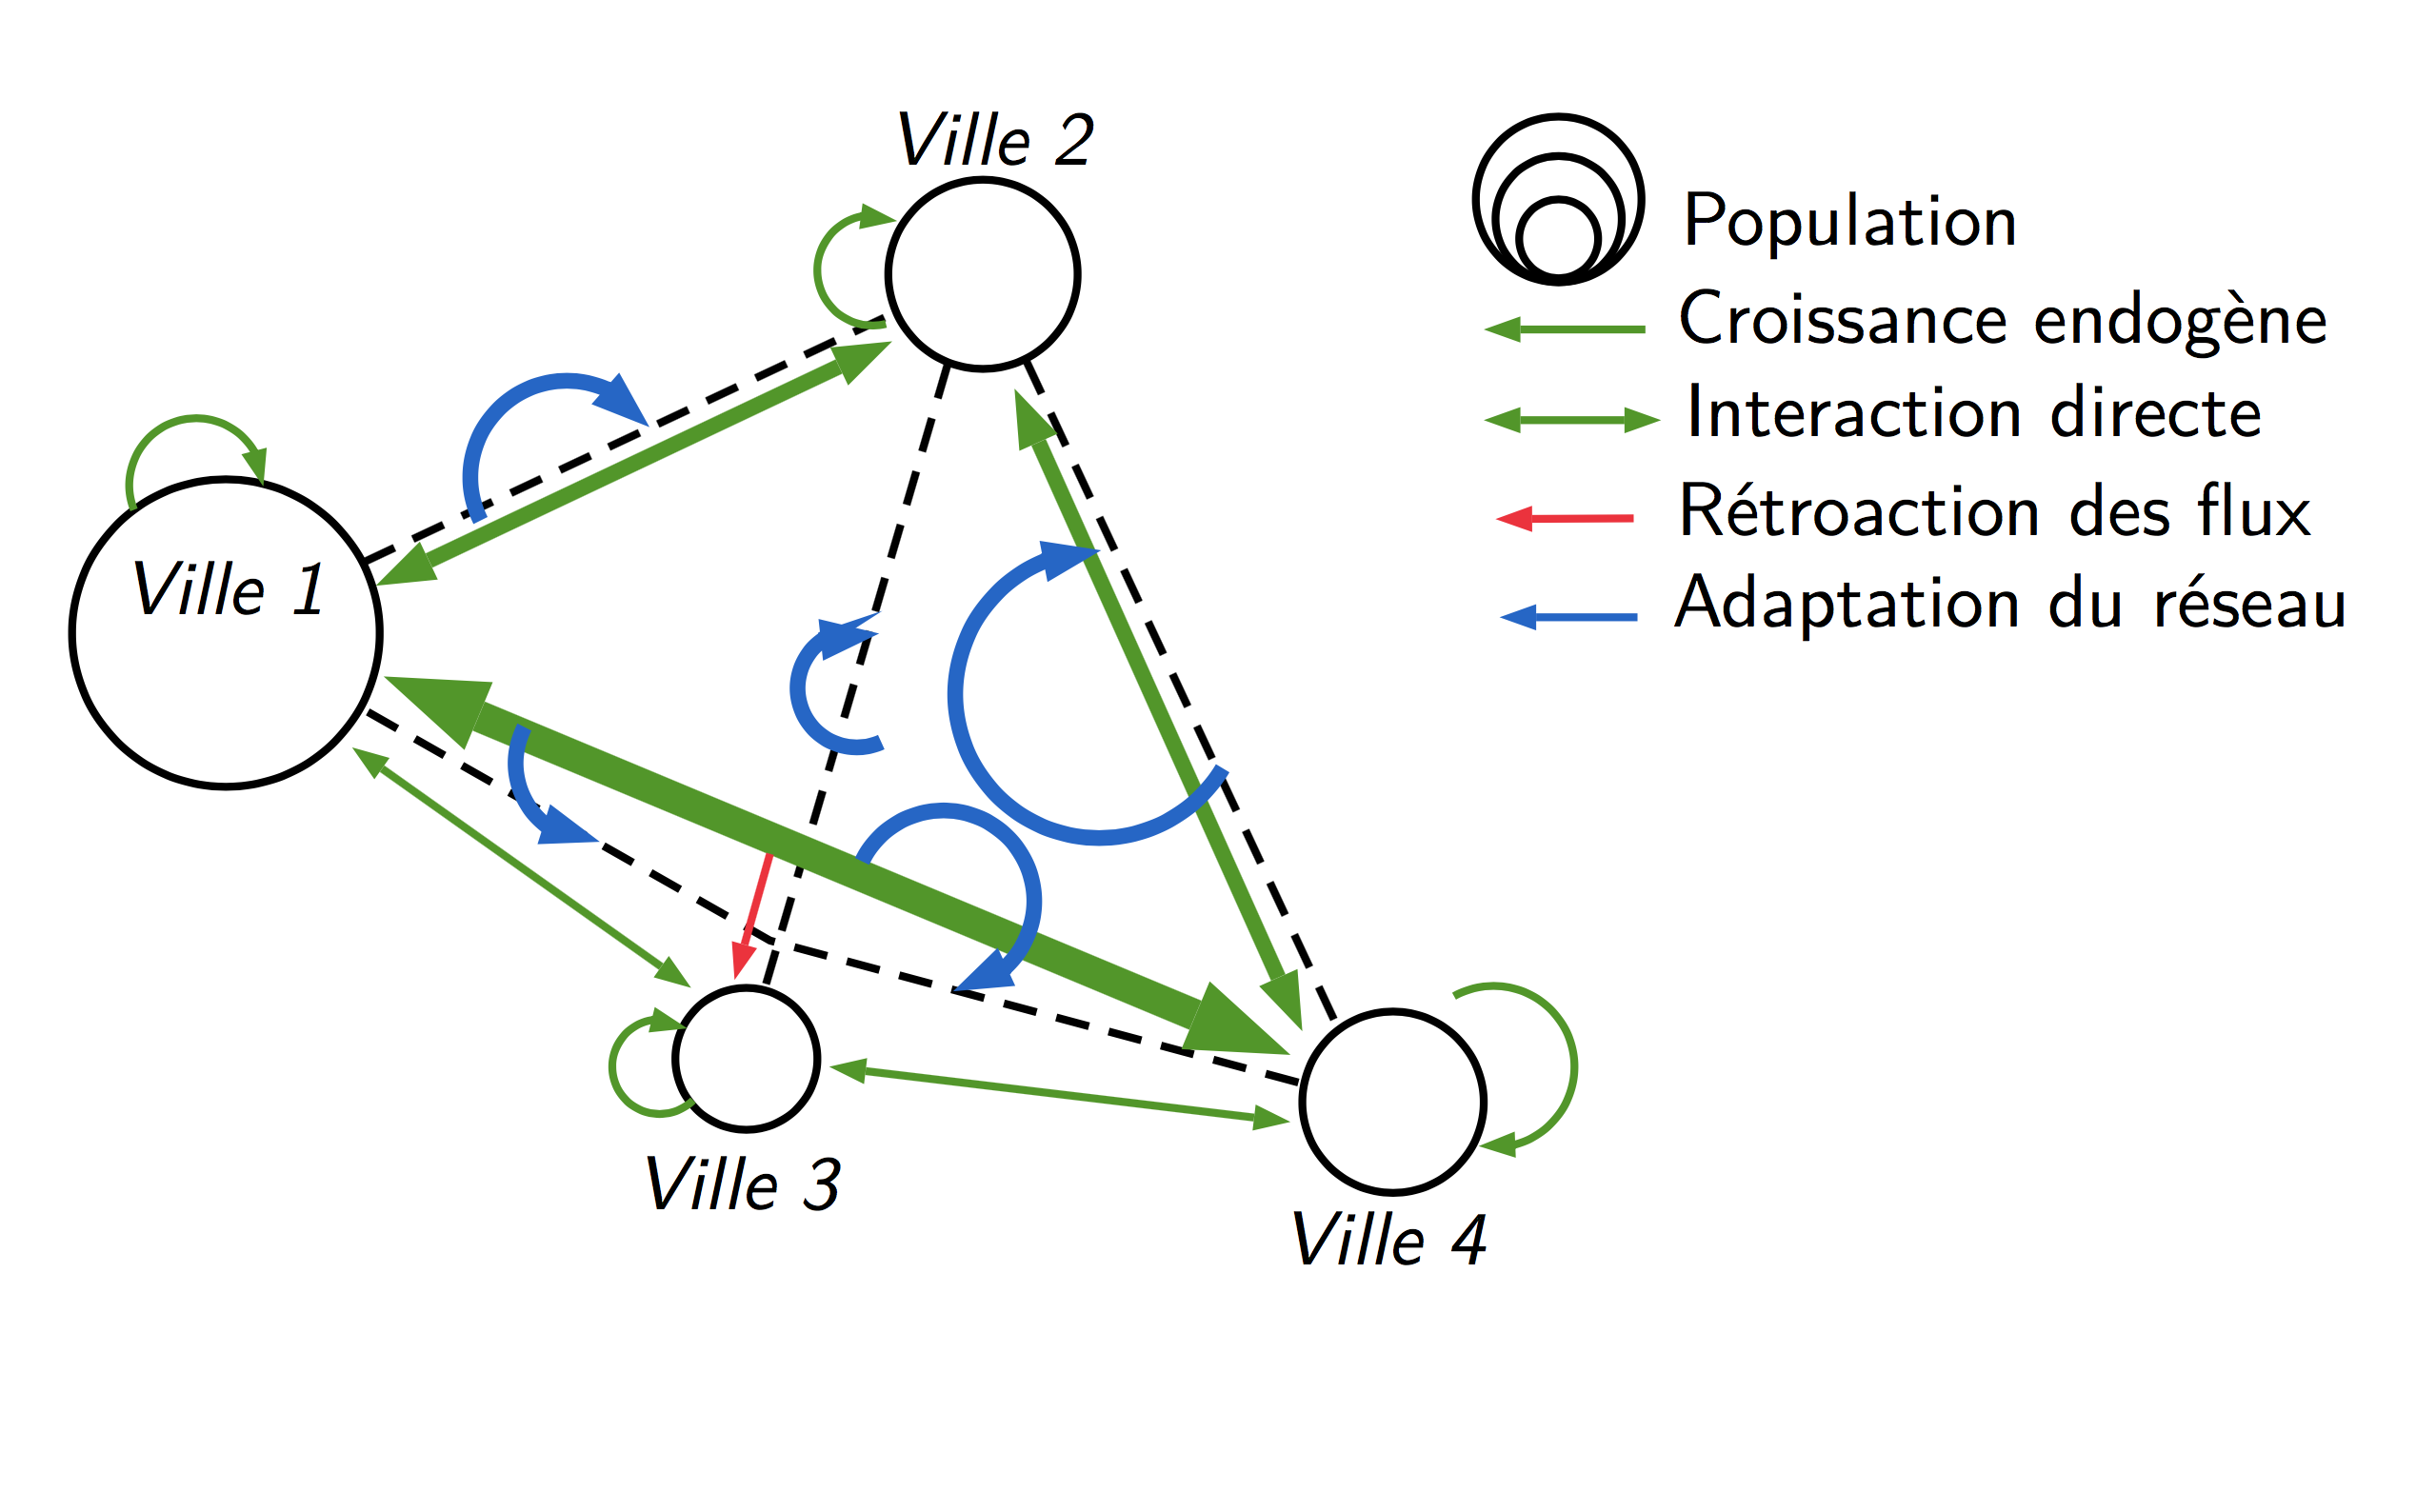
\includegraphics[width=\textwidth]{figures/macrocoevol_model.png}


\nocite{raimbault2018indirect}
\nocite{raimbault2019modeling}

\vspace{-1cm}

\footnotesize

Raimbault, J. (2018). Indirect evidence of network effects in a system of cities. Environment and Planning B: Urban Analytics and City Science, 2399808318774335.

\smallskip

Raimbault, J. (2019). Modeling the co-evolution of cities and networks. In Niel, Z., Rozenblat, C., eds. \textit{Handbook of Cities and Network}, Edwar Elgar Publishing, \textit{in press}.


}



\sframe{Modèles macroscopiques : régimes de co-évolution}{

%\begin{column}{0.3\textwidth}

\centering

	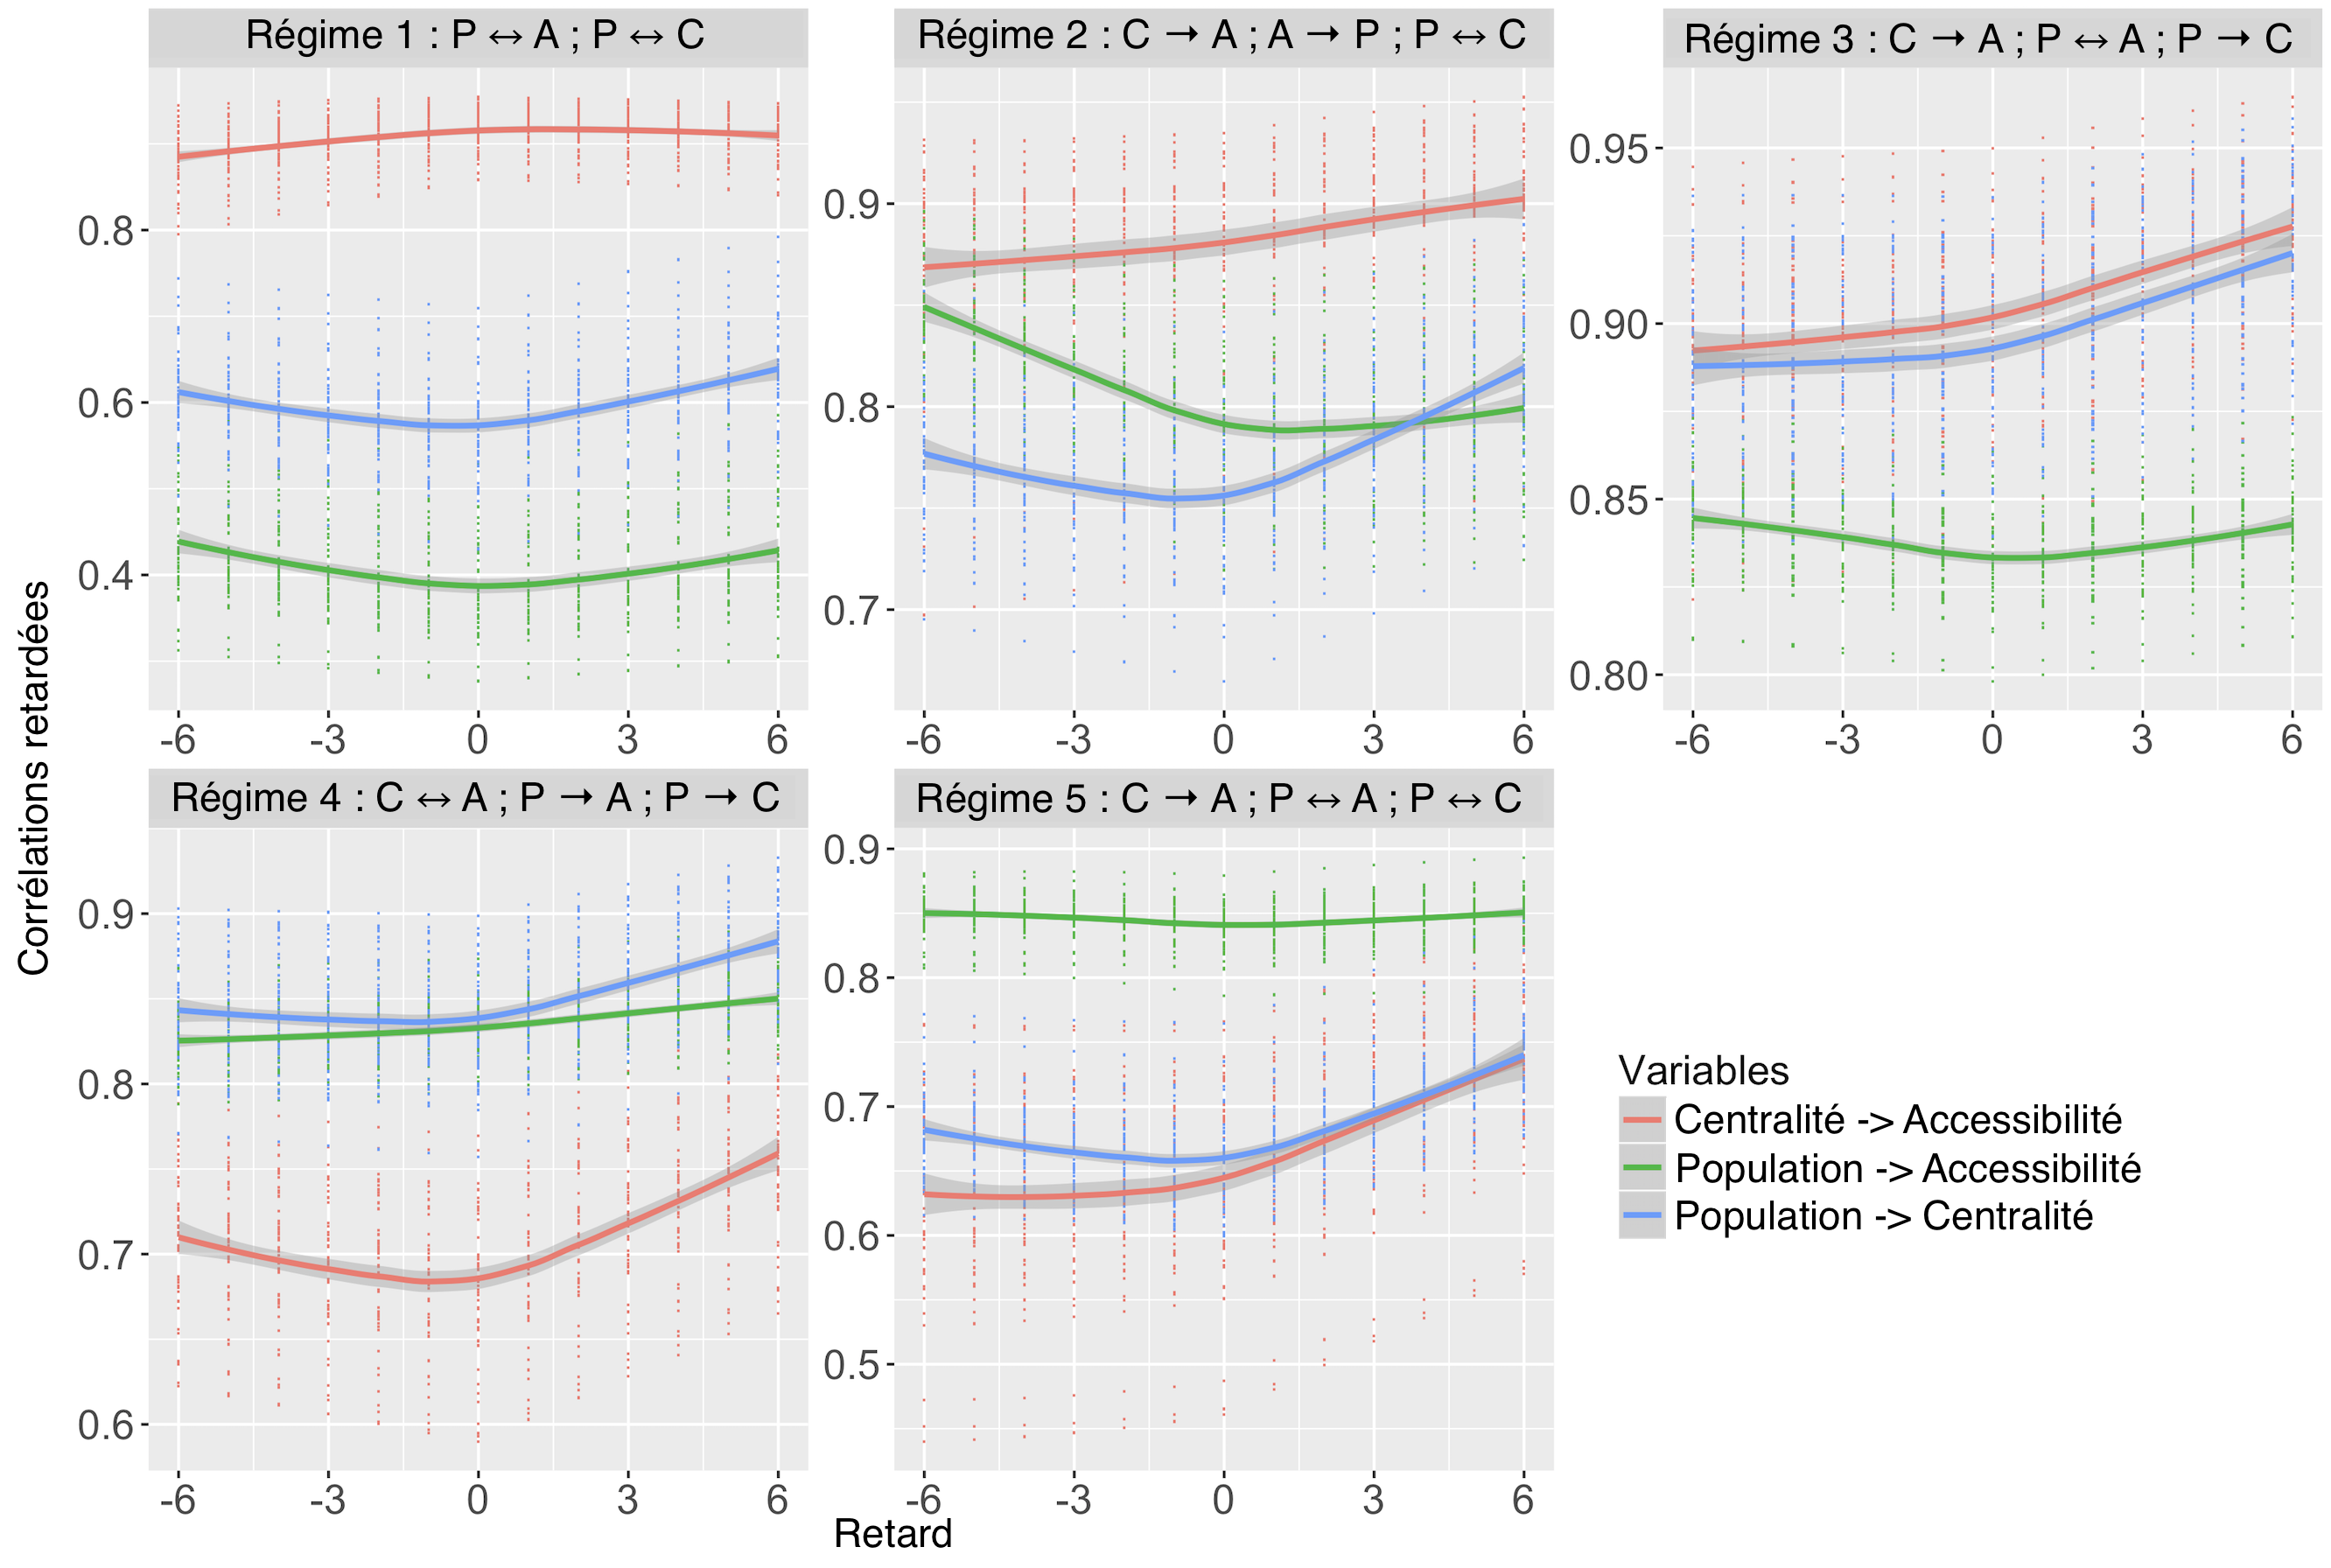
\includegraphics[width=\linewidth]{figures/macro-regimes.png}
	
	\medskip
	
	%\footnotesize
	
	%\begin{justify}

\raggedleft

\vspace{-0.4cm}

	\textit{Multiples régimes mis en évidence dans des configurations synthétiques}


	%\end{justify}
%\end{column}


}








%%%%%
%% Slide meso
%%%%%

\sframe{Modèles mésoscopiques: morphogenèse}{


% - complementarité de multiples heuristiques de croissance de reseau
% - calibration au premier et second ordre
% - Lutecia : vers des modèles plus complexes


\footnotesize

%Relation entre forme et fonction (morphogenèse) comme paradigme pour modéliser la co-évolution à l'échelle mésoscopique.

%\smallskip

%\begin{columns}
%\begin{column}{0.55\textwidth}

%\footnotesize

\vspace{-0.8cm}

\justify
\textit{Un modèle par réaction-diffusion et multi-modélisation de la croissance du réseau : complémentarité des heuristiques, calibration sur les formes et leurs corrélations}

\medskip

{\centering
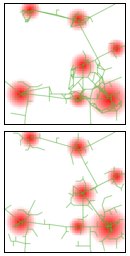
\includegraphics[width=0.25\linewidth,height=0.6\textheight]{figures/meso-nwgrowth.png}
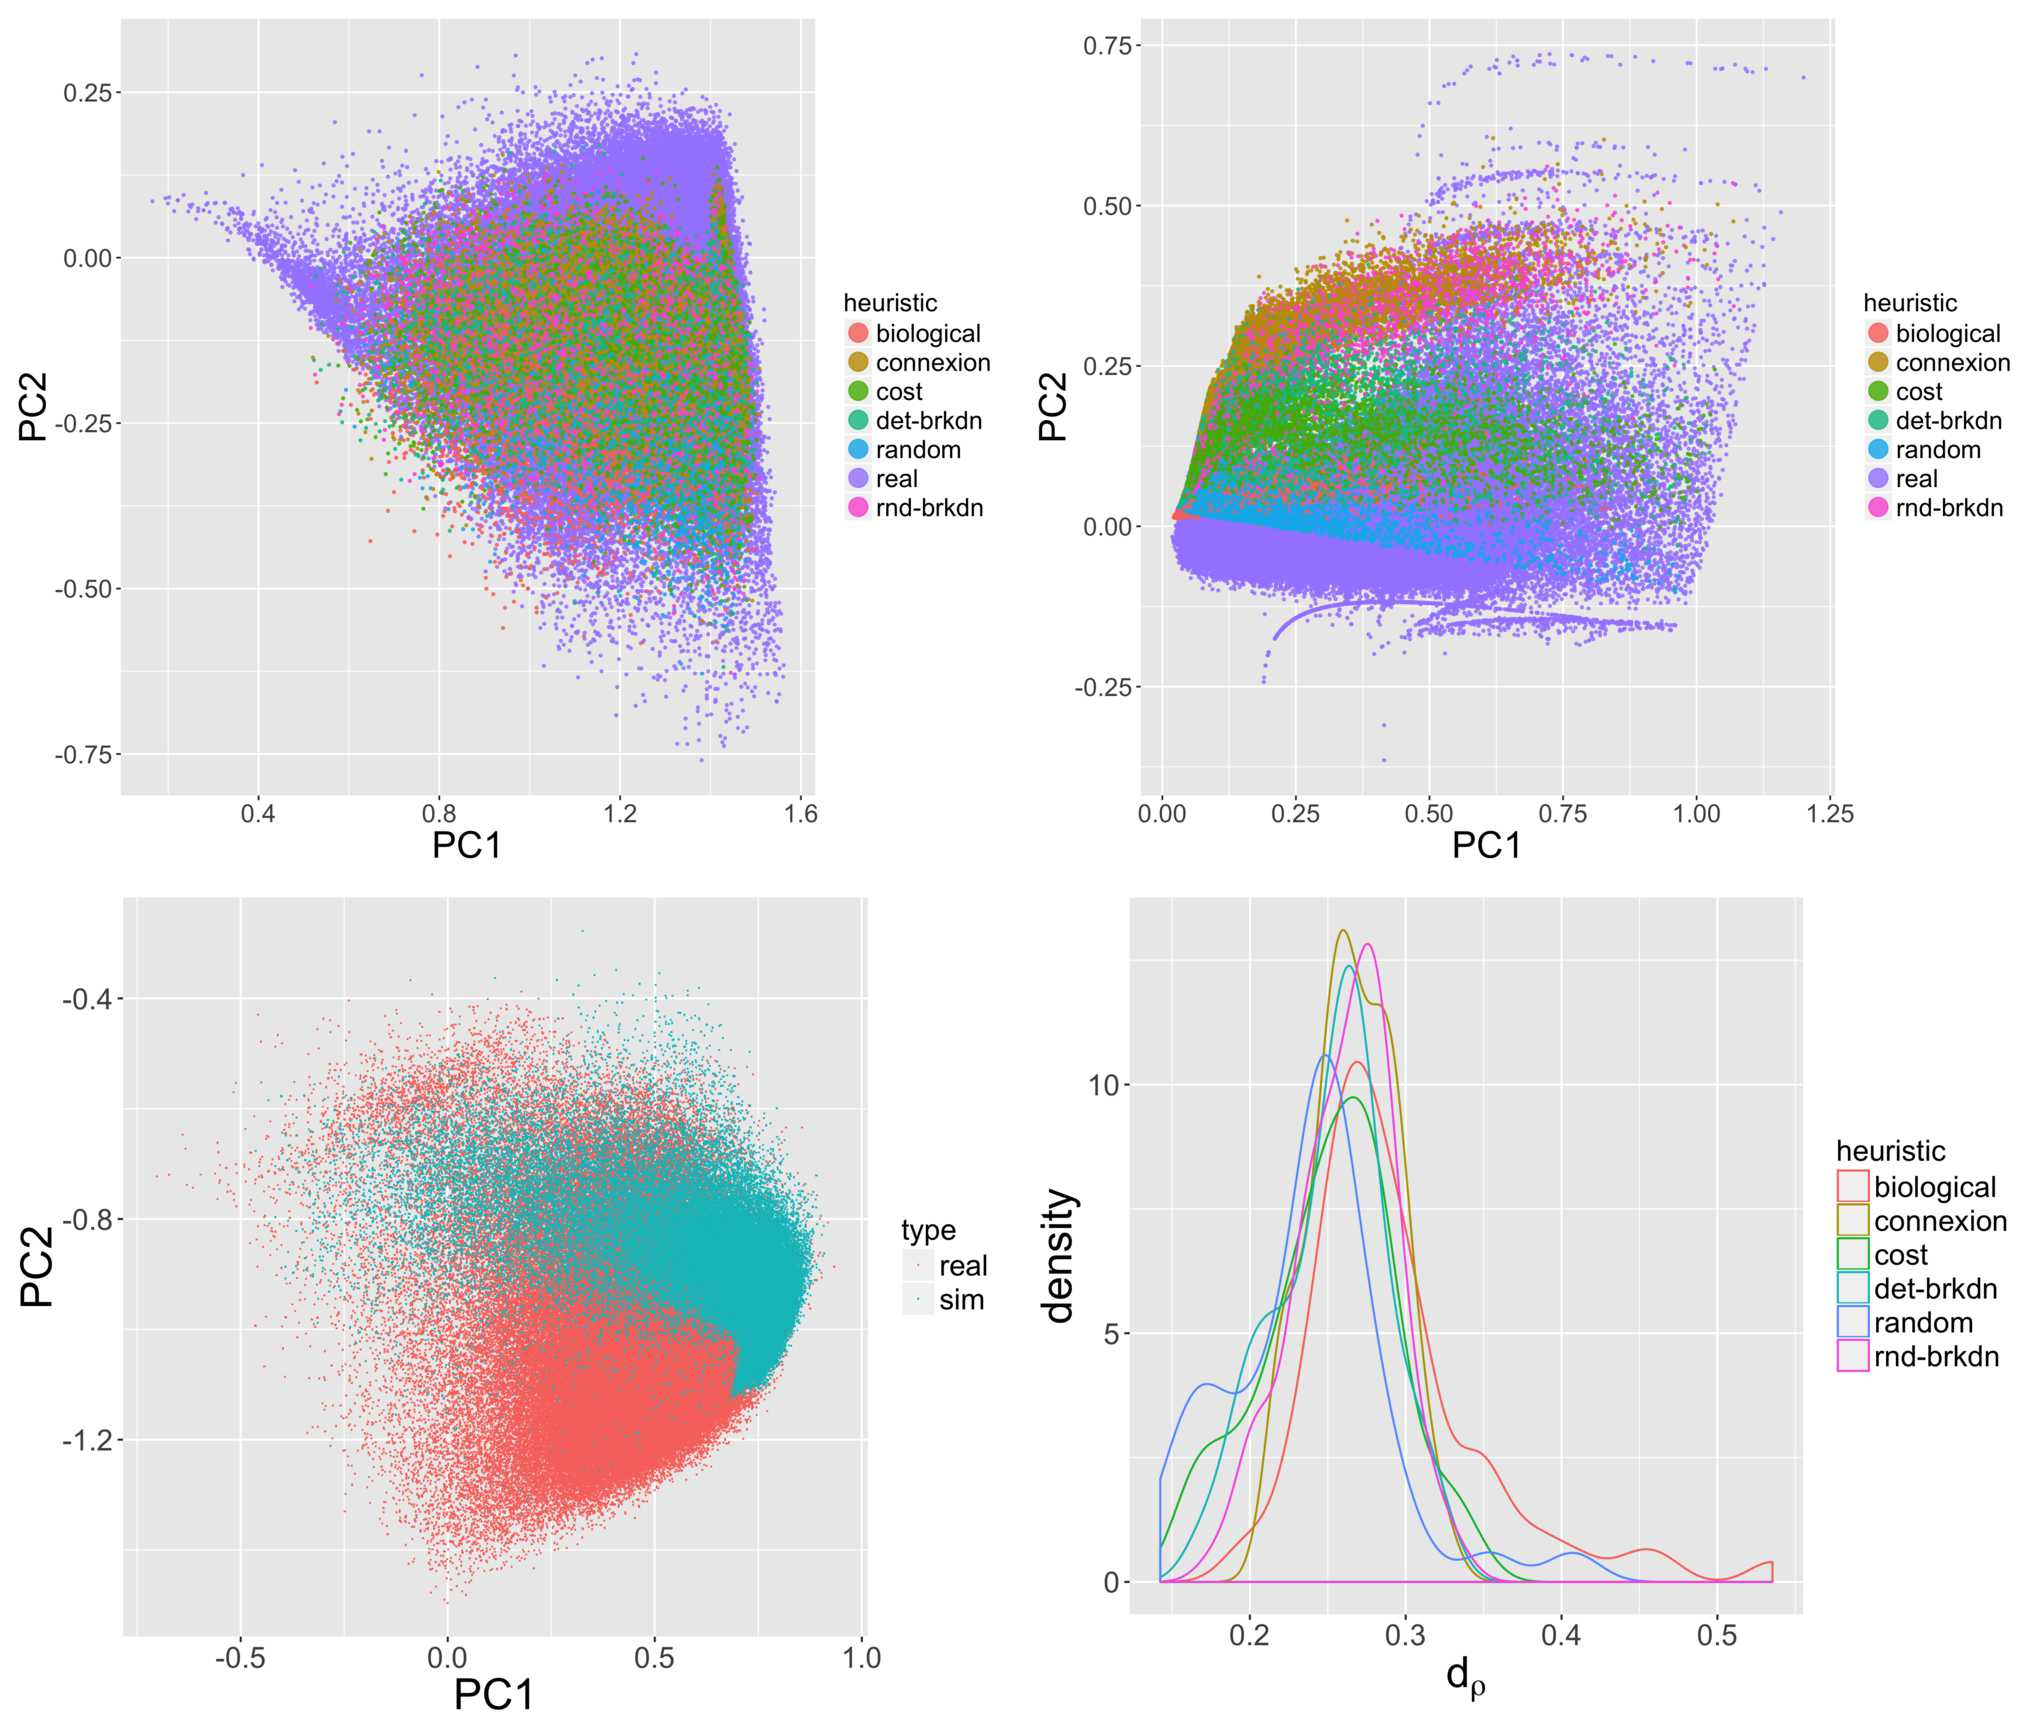
\includegraphics[width=0.6\linewidth,height=0.6\textheight]{figures/meso-calib.jpg}
}

%\medskip

%$\rightarrow$ \textit{Complémentarité des heuristiques de réseau}
%  pour reproduire des formes existantes

%$\rightarrow$ \textit{Calibration sur les formes et leurs corrélations}

%\end{column}
%\vrule
%\hspace{0.2cm}
%\begin{column}{0.35\textwidth}

%\footnotesize

\bigskip

\tiny

Raimbault, J. (2018). Calibration of a density-based model of urban morphogenesis. PloS one, 13(9), e0203516.

\nocite{raimbault2018calibration}

\smallskip

Raimbault, J. (2019). An urban morphogenesis model capturing interactions between networks and territories. In The Mathematics of Urban Morphology (pp. 383-409). Birkhäuser, Cham.

\nocite{raimbault2019urban}




}


%
\sframe{Modèles mésoscopiques}{


\textit{Le modèle Lutecia : vers une prise en compte de la gouvernance pour la croissance des réseaux de transport}

\bigskip

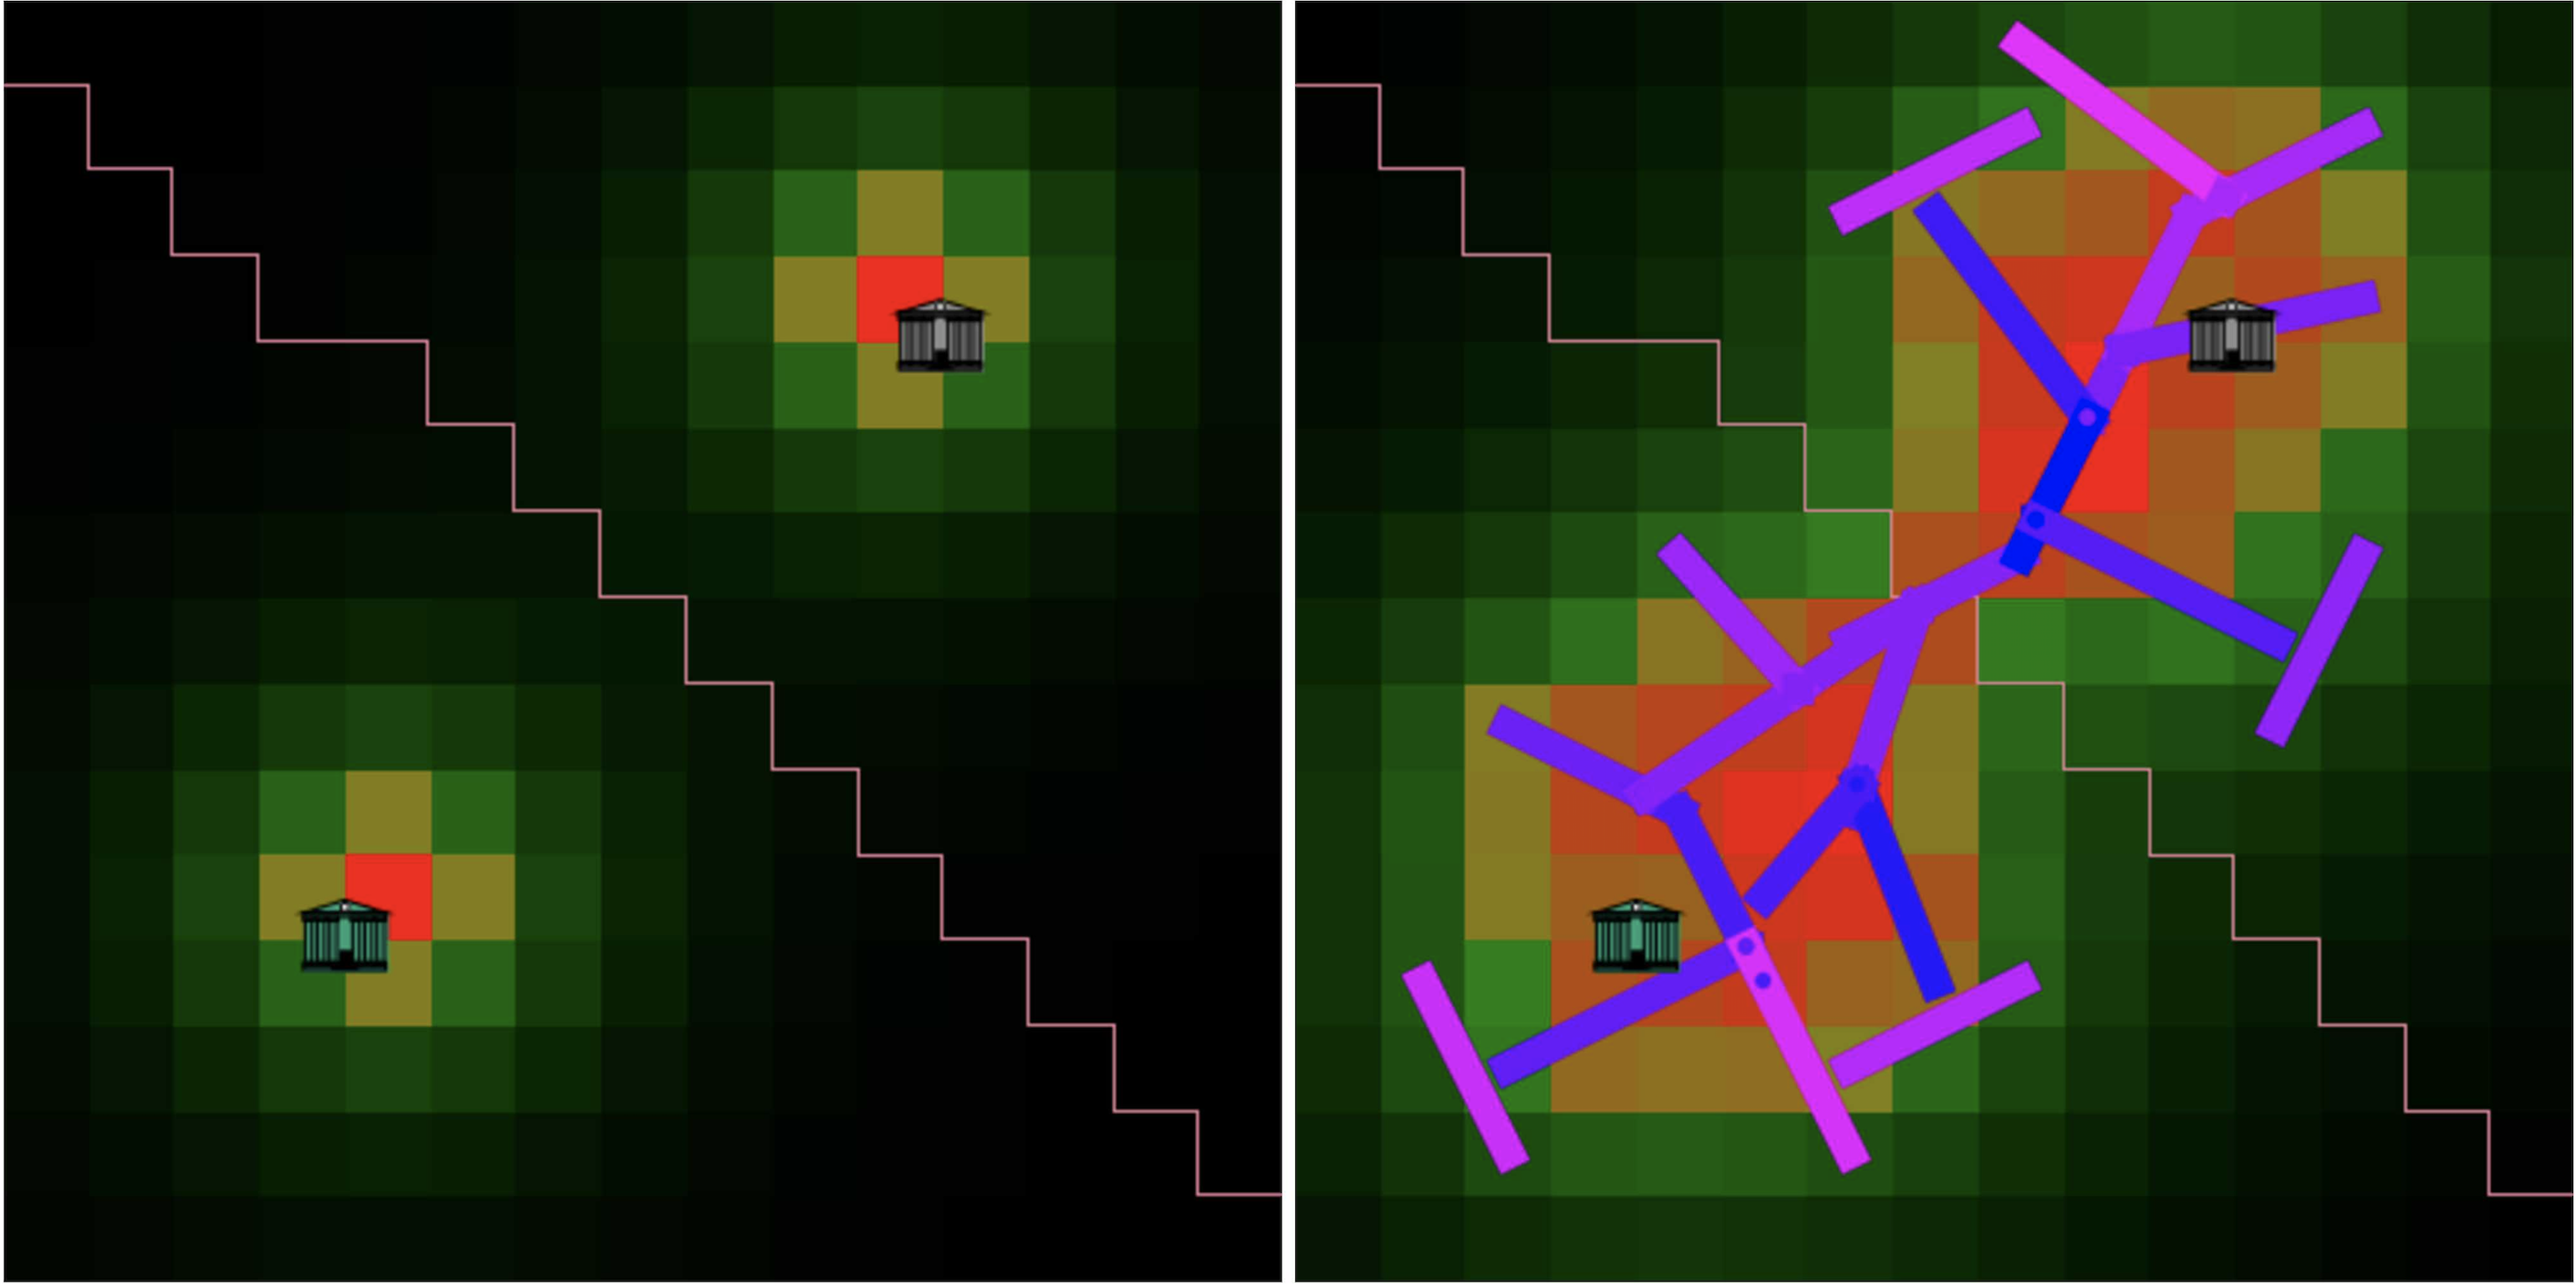
\includegraphics[width=\linewidth]{figures/meso-lutecia.jpg}




%\end{column}
%\end{columns}


}



\sframe{Ouvertures}{

% Vers des théories intégratives des systèmes territoriaux

% donner des pistes
% theorique, epistemo quanti
% ici parler des developpements Lutecia : modeles.
% multi-modeling
%. -> bien parler de tous les domaines.
%. certains elements plus tangibles : va dans le sens de Morency : compris que quelque chose ici. : strqtgeie explorqtion ; redeveloppement langages scalable. : fait comprendre que chapitre creuser pas possible tel quel, passage a l'echelle necessaire, etc.
% 
% slide de fin : riche, permet ouverture.
%
% 

\textbf{Contributions}

\begin{itemize}
	\item \textit{Définition :} relecture possible de la théorie évolutive, ouvre \\
	 des ponts vers l'économie géographique
	\item \textit{Caractérisation : } nombreuses perspectives d'applications\\
	 en géographie, en sciences territoriales
	\item \textit{Modélisation : } des modèles interdisciplinaires ayant vocation\\
	à être couplés et réutilisés
\end{itemize}

\bigskip

\uncover<2->{

\textbf{Perspectives}

\begin{itemize}
	\item Adaptation de Lutecia pour le développement de méthodes d'exploration de modèles spatiaux (développement d'OpenMole)
	\item \textit{Vers des théories intégrées des systèmes territoriaux : } modèles multi-échelles et couplage de la théorie évolutive avec la théorie \\
	 du \textit{Scaling}.
\end{itemize}
}

}




\sframe{Problématique et plan dans les domaines de connaissance}{

\centering
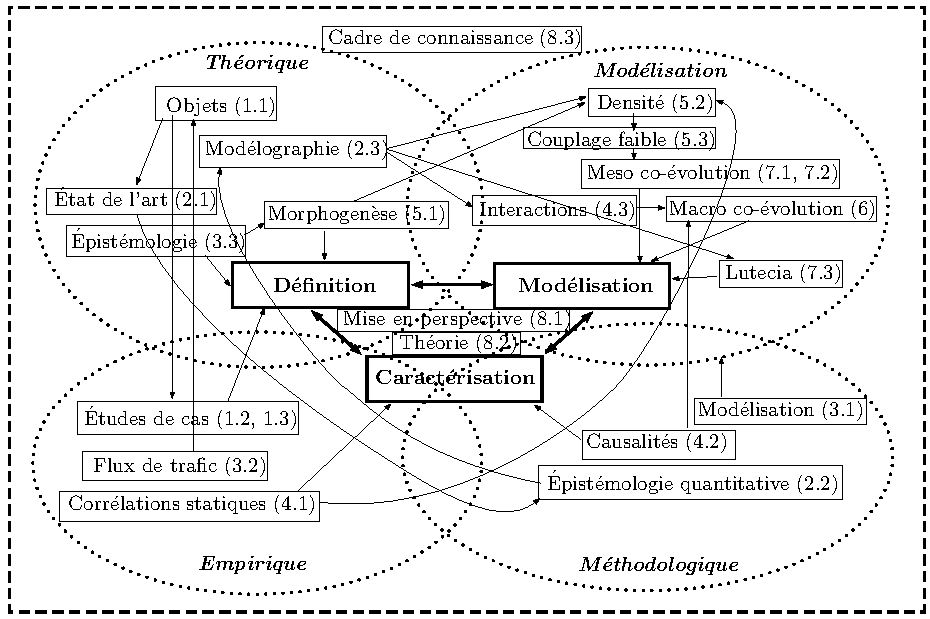
\includegraphics[width=\linewidth]{figures/domconn-organisation.pdf}

}







\sframe{Mise en perspective}{
\centering

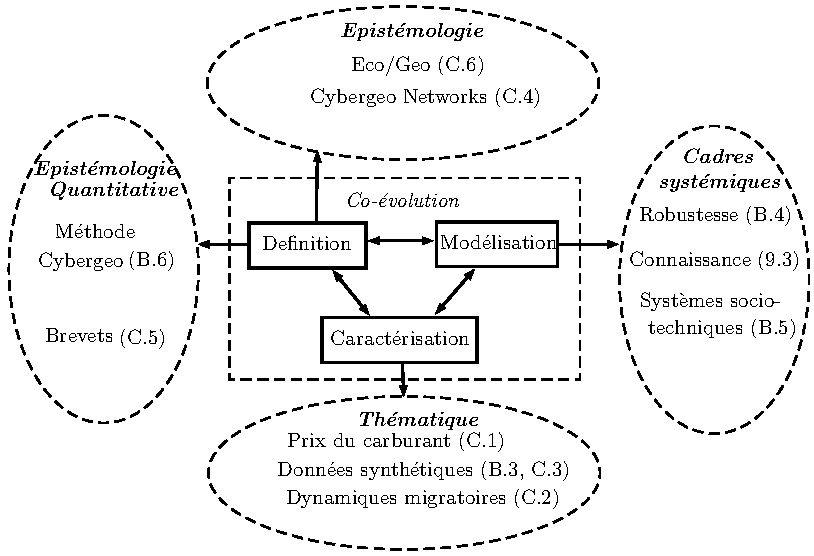
\includegraphics[width=\linewidth]{figures/opening-meta.pdf}

}


\sframe{Analyse réflexive}{

\centering

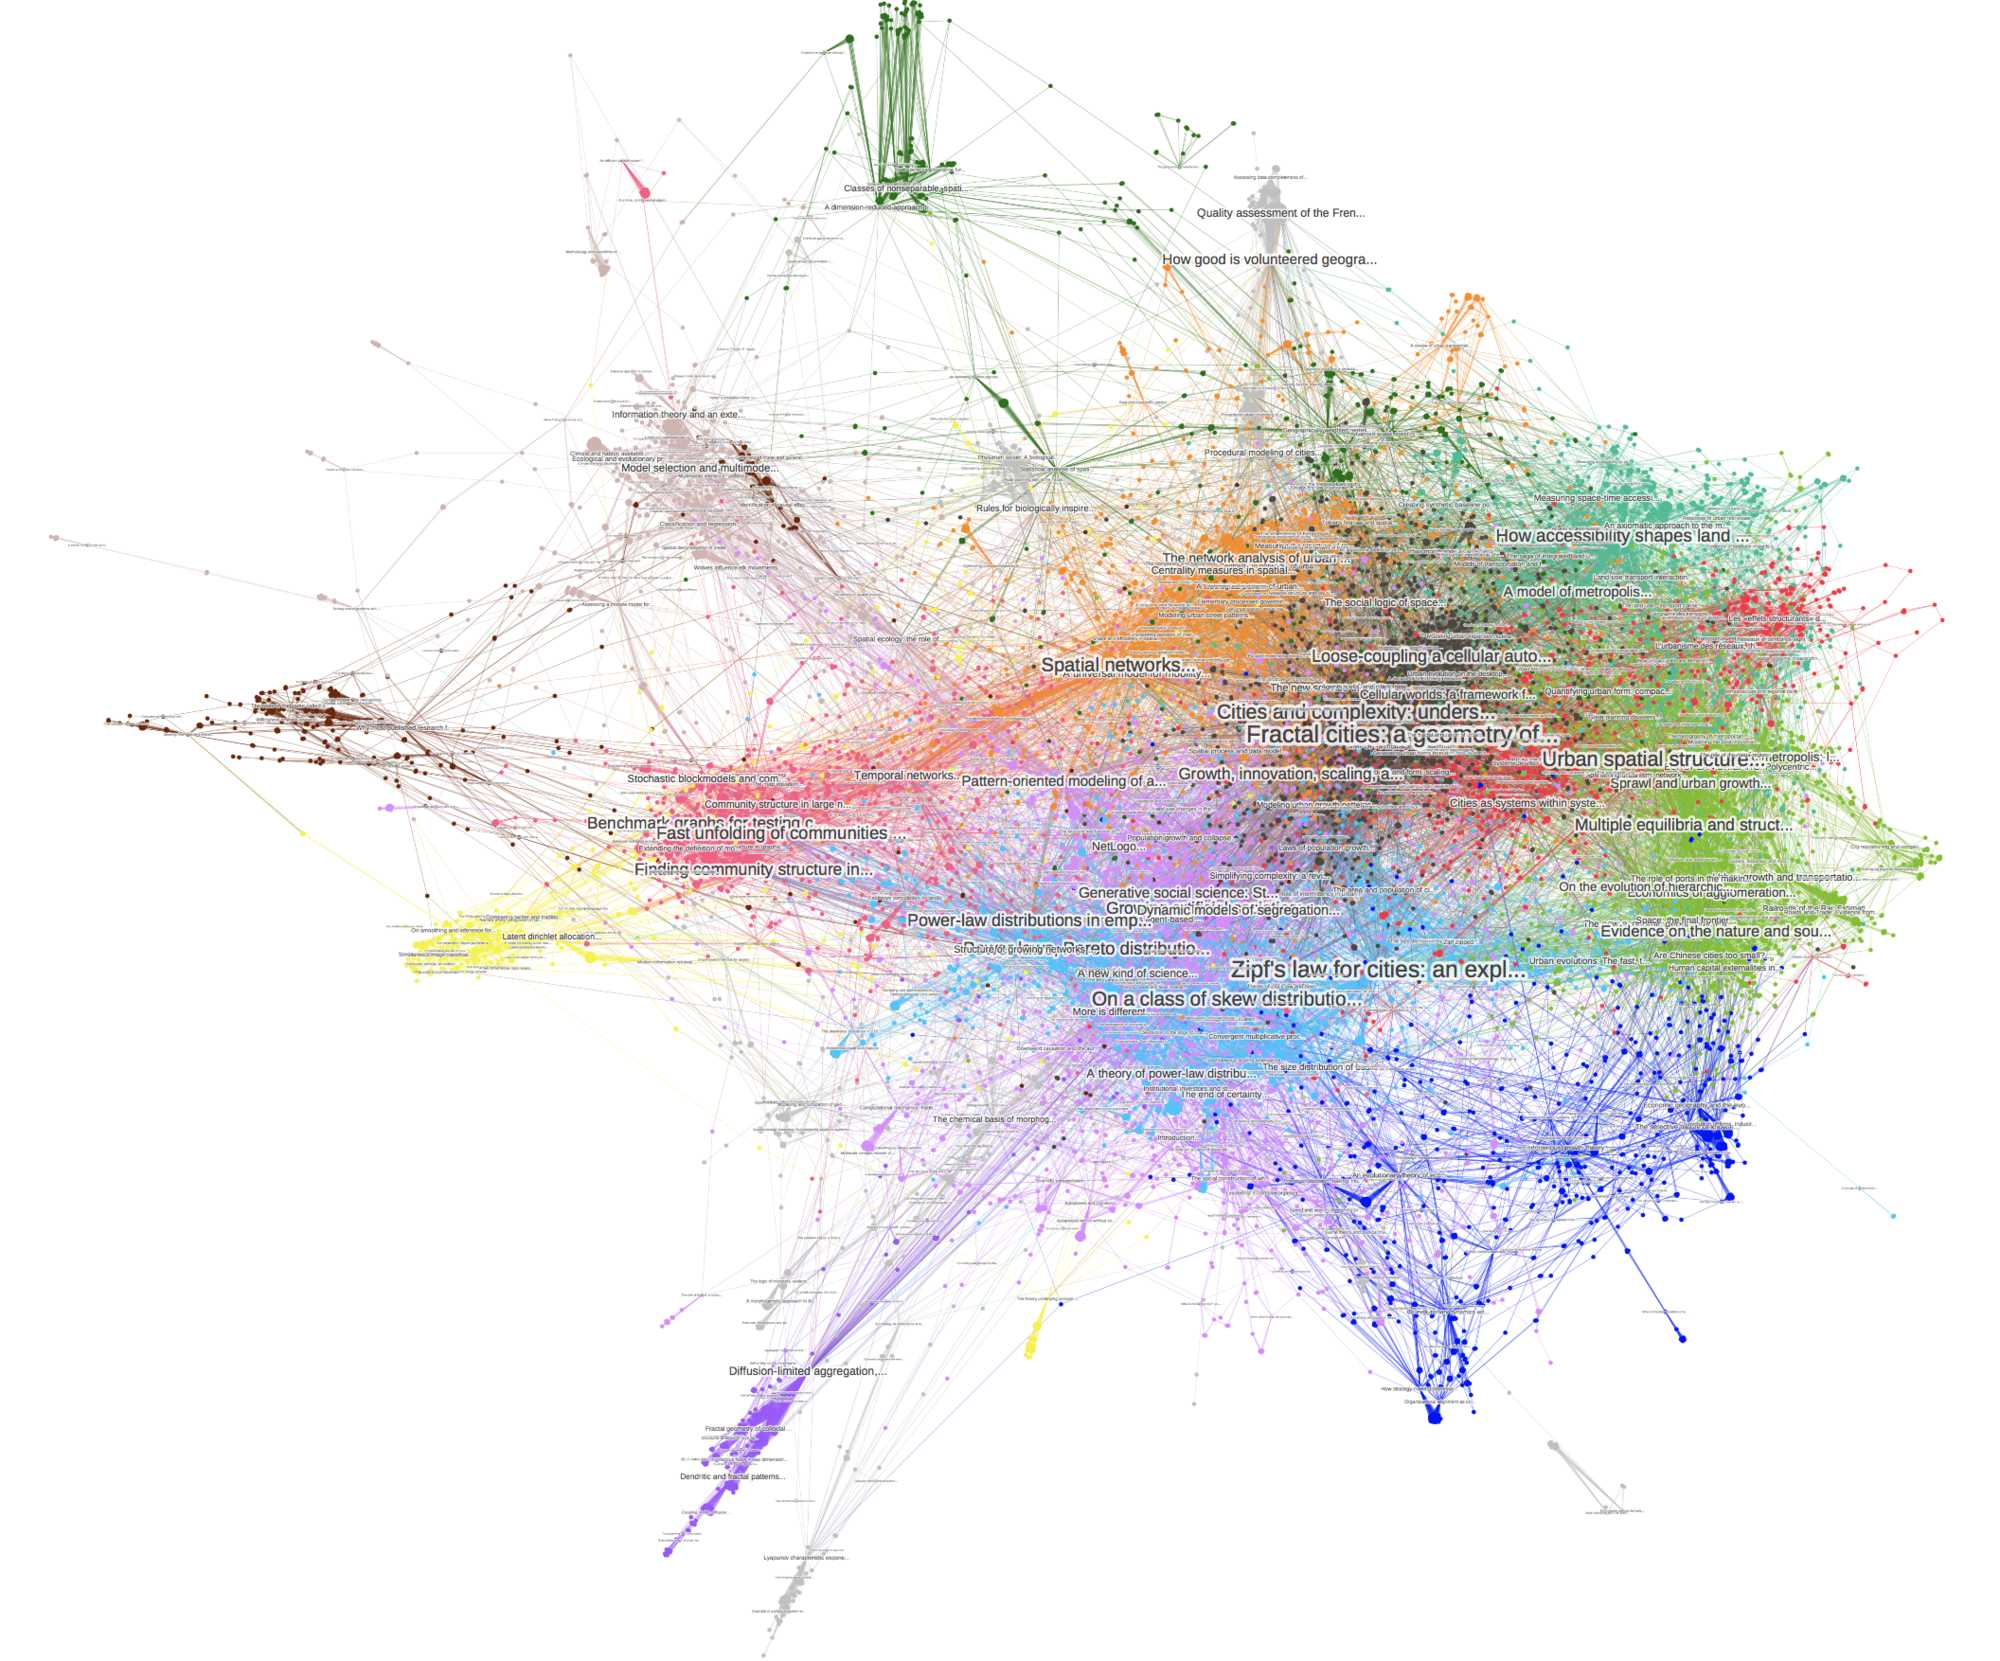
\includegraphics[width=0.9\textwidth]{figures/F-reflexivity-citnw.jpg}

}

\sframe{Conclusion: contributions Systèmes Complexes}{

\justify

\vspace{-1cm}

\textbf{Interdisciplinarité}

\medskip

$\rightarrow$ Outils ouverts d'épistémologie quantitative et d'analyse réflexive

\smallskip

$\rightarrow$ Ponts entre disciplines: géographie, transports, économie, \textit{Artificial Life}, épistémologie quantitative

\bigskip

\textbf{Méthodologie}

\medskip

$\rightarrow$ Analyse empirique de systèmes spatio-temporels

\smallskip

$\rightarrow$ Méthodes d'exploration de modèles (analyse de sensibilité spatiale)

\bigskip

\textbf{Complexité}

\medskip

$\rightarrow$ Etude interdisciplinaire de concepts clés (morphogenèse, co-évolution)

\smallskip

$\rightarrow$ Liens entre complexités

\smallskip

$\rightarrow$ Cadres d'étude en complexité





}





%%%%%%%%%%%%%%%%%%%%%
\begin{frame}[allowframebreaks]
\frametitle{References}
\bibliographystyle{apalike}
\bibliography{/Users/juste/ComplexSystems/CityNetwork/Biblio/Bibtex/CityNetwork,biblio}
\end{frame}
%%%%%%%%%%%%%%%%%%%%%%%%%%%%



\end{document}







